% arXiv version of the shared-board write-up. Structure follows the ORQA arXiv paper:
% Abstract, 1 Introduction, 2 Related Work, 3 Methodology, 4 Results, 5 Discussion, References, Appendix.
% Every number in the text is a macro from tables/numbers.tex, generated by
% paper/scripts/arxiv_sharing_tables.py from the result files; the tables are generated by the same script.
\documentclass[11pt]{article}
\usepackage[margin=1in]{geometry}
\usepackage{times}
\usepackage[T1]{fontenc}
\usepackage[utf8]{inputenc}
\usepackage{microtype}
\usepackage{amsmath,amssymb}
\usepackage{graphicx}
\usepackage{booktabs}
\usepackage{array}
\usepackage{float}
\usepackage{placeins}
\usepackage{xcolor}
\usepackage[round]{natbib}
\usepackage{enumitem}
\usepackage{caption}
\usepackage{hyperref}
\hypersetup{colorlinks=true, linkcolor=blue!60!black, citecolor=blue!60!black, urlcolor=blue!60!black}
\usepackage{url}

% GENERATED by paper/scripts/arxiv_sharing_tables.py; do not edit.
\newcommand{\NWorlds}{8}
\newcommand{\NAgents}{3}
\newcommand{\NRounds}{20}
\newcommand{\NAttempts}{60}
\newcommand{\LemSoloMax}{84.4}
\newcommand{\LemShareMax}{75.4}
\newcommand{\AliSoloMax}{86.8}
\newcommand{\AliShareMax}{71.2}
\newcommand{\LemSoloSum}{53.7}
\newcommand{\LemShareSum}{64.9}
\newcommand{\AliSoloSum}{48.4}
\newcommand{\AliShareSum}{58.8}
\newcommand{\LemSoloUniq}{42.8}
\newcommand{\LemShareUniq}{22.8}
\newcommand{\AliSoloUniq}{48.0}
\newcommand{\AliShareUniq}{25.1}
\newcommand{\AliPeriodicMax}{89.7}
\newcommand{\AliProtocolMax}{88.3}
\newcommand{\LemPeriodicMax}{78.8}
\newcommand{\LemProtocolMax}{78.5}
\newcommand{\LemStaggerSum}{72.1}
\newcommand{\AliProtocolSum}{67.3}
\newcommand{\OwnBestLem}{+8.5}
\newcommand{\OwnBestAli}{+9.9}
\newcommand{\SameLocSoloLem}{30}
\newcommand{\SameLocShareLem}{96}
\newcommand{\SameLocSoloAli}{33}
\newcommand{\SameLocShareAli}{94}
\newcommand{\AllLemMax}{-8.5}
\newcommand{\AllLemMaxLo}{-21.9}
\newcommand{\AllLemMaxHi}{+4.8}
\newcommand{\AllLemMaxP}{0.219}
\newcommand{\AllLemSum}{+8.7}
\newcommand{\AllLemSumLo}{+4.1}
\newcommand{\AllLemSumHi}{+13.2}
\newcommand{\AllLemSumP}{0.016}
\newcommand{\AllLemUniq}{-12.9}
\newcommand{\AllLemUniqLo}{-17.6}
\newcommand{\AllLemUniqHi}{-8.2}
\newcommand{\AllLemUniqP}{0.008}
\newcommand{\AllAliMax}{-6.6}
\newcommand{\AllAliMaxLo}{-17.6}
\newcommand{\AllAliMaxHi}{+4.4}
\newcommand{\AllAliMaxP}{0.227}
\newcommand{\AllAliSum}{+11.0}
\newcommand{\AllAliSumLo}{+7.7}
\newcommand{\AllAliSumHi}{+14.3}
\newcommand{\AllAliSumP}{0.008}
\newcommand{\AllAliUniq}{-14.5}
\newcommand{\AllAliUniqLo}{-17.2}
\newcommand{\AllAliUniqHi}{-11.7}
\newcommand{\AllAliUniqP}{0.008}
\newcommand{\AllBothMax}{-7.6}
\newcommand{\AllBothMaxLo}{-17.9}
\newcommand{\AllBothMaxHi}{+2.7}
\newcommand{\AllBothMaxP}{0.109}
\newcommand{\AllBothSum}{+9.8}
\newcommand{\AllBothSumLo}{+6.9}
\newcommand{\AllBothSumHi}{+12.7}
\newcommand{\AllBothSumP}{0.008}
\newcommand{\AllBothUniq}{-13.7}
\newcommand{\AllBothUniqLo}{-16.2}
\newcommand{\AllBothUniqHi}{-11.2}
\newcommand{\AllBothUniqP}{0.008}
\newcommand{\AliPeriodicDiff}{+2.9}
\newcommand{\AliPeriodicLo}{-12.7}
\newcommand{\AliPeriodicHi}{+18.5}
\newcommand{\AliPeriodicP}{0.70}
\newcommand{\AliProtocolDiff}{+1.5}
\newcommand{\AliProtocolP}{0.84}
\newcommand{\AliPeriodicReached}{20 of 24}
\newcommand{\AliSoloReached}{19 of 24}
\newcommand{\LemSoloReached}{17 of 24}
\newcommand{\LemShareReached}{12 of 24}
\newcommand{\AliShareReached}{12 of 24}
\newcommand{\AgreeSame}{44}
\newcommand{\AgreeOf}{48}
\newcommand{\WNewMax}{-0.6}
\newcommand{\WNewMaxLo}{-4.8}
\newcommand{\WNewMaxHi}{+3.5}
\newcommand{\WNewMaxP}{=0.875}
\newcommand{\WNewMaxDown}{2}
\newcommand{\WNewMaxUp}{2}
\newcommand{\WNewMaxSolo}{90.8}
\newcommand{\WNewMaxArm}{90.2}
\newcommand{\WNewMaxN}{16}
\newcommand{\WAllMax}{+0.6}
\newcommand{\WAllMaxLo}{-4.6}
\newcommand{\WAllMaxHi}{+5.7}
\newcommand{\WAllMaxP}{=0.838}
\newcommand{\WAllMaxDown}{4}
\newcommand{\WAllMaxUp}{7}
\newcommand{\WAllMaxSolo}{89.5}
\newcommand{\WAllMaxArm}{90.0}
\newcommand{\WAllMaxN}{24}
\newcommand{\WPilotMax}{+2.9}
\newcommand{\WPilotMaxLo}{-12.7}
\newcommand{\WPilotMaxHi}{+18.5}
\newcommand{\WPilotMaxP}{=0.703}
\newcommand{\WPilotMaxDown}{2}
\newcommand{\WPilotMaxUp}{5}
\newcommand{\WPilotMaxSolo}{86.8}
\newcommand{\WPilotMaxArm}{89.7}
\newcommand{\WPilotMaxN}{8}
\newcommand{\WNewSum}{+5.9}
\newcommand{\WNewSumLo}{+2.5}
\newcommand{\WNewSumHi}{+9.4}
\newcommand{\WNewSumP}{=0.002}
\newcommand{\WNewSumDown}{3}
\newcommand{\WNewSumUp}{13}
\newcommand{\WNewSumSolo}{63.0}
\newcommand{\WNewSumArm}{68.9}
\newcommand{\WNewSumN}{16}
\newcommand{\WAllSum}{+7.8}
\newcommand{\WAllSumLo}{+4.7}
\newcommand{\WAllSumHi}{+10.9}
\newcommand{\WAllSumP}{<0.001}
\newcommand{\WAllSumDown}{4}
\newcommand{\WAllSumUp}{20}
\newcommand{\WAllSumSolo}{58.1}
\newcommand{\WAllSumArm}{65.9}
\newcommand{\WAllSumN}{24}
\newcommand{\WPilotSum}{+11.5}
\newcommand{\WPilotSumLo}{+4.9}
\newcommand{\WPilotSumHi}{+18.1}
\newcommand{\WPilotSumP}{=0.016}
\newcommand{\WPilotSumDown}{1}
\newcommand{\WPilotSumUp}{7}
\newcommand{\WPilotSumSolo}{48.4}
\newcommand{\WPilotSumArm}{59.9}
\newcommand{\WPilotSumN}{8}
\newcommand{\WNewUniq}{-7.5}
\newcommand{\WNewUniqLo}{-9.2}
\newcommand{\WNewUniqHi}{-5.8}
\newcommand{\WNewUniqP}{<0.001}
\newcommand{\WNewUniqDown}{16}
\newcommand{\WNewUniqUp}{0}
\newcommand{\WNewUniqSolo}{46.1}
\newcommand{\WNewUniqArm}{38.6}
\newcommand{\WNewUniqN}{16}
\newcommand{\WAllUniq}{-6.7}
\newcommand{\WAllUniqLo}{-8.2}
\newcommand{\WAllUniqHi}{-5.2}
\newcommand{\WAllUniqP}{<0.001}
\newcommand{\WAllUniqDown}{23}
\newcommand{\WAllUniqUp}{1}
\newcommand{\WAllUniqSolo}{46.8}
\newcommand{\WAllUniqArm}{40.0}
\newcommand{\WAllUniqN}{24}
\newcommand{\WPilotUniq}{-5.2}
\newcommand{\WPilotUniqLo}{-8.6}
\newcommand{\WPilotUniqHi}{-1.9}
\newcommand{\WPilotUniqP}{=0.023}
\newcommand{\WPilotUniqDown}{7}
\newcommand{\WPilotUniqUp}{1}
\newcommand{\WPilotUniqSolo}{48.0}
\newcommand{\WPilotUniqArm}{42.8}
\newcommand{\WPilotUniqN}{8}
\newcommand{\WNewReached}{-2.1}
\newcommand{\WNewReachedLo}{-12.3}
\newcommand{\WNewReachedHi}{+8.1}
\newcommand{\WNewReachedP}{=1.000}
\newcommand{\WNewReachedDown}{1}
\newcommand{\WNewReachedUp}{1}
\newcommand{\WNewReachedSolo}{83.3}
\newcommand{\WNewReachedArm}{81.2}
\newcommand{\WNewReachedN}{16}
\newcommand{\WAllReached}{-0.0}
\newcommand{\WAllReachedLo}{-10.2}
\newcommand{\WAllReachedHi}{+10.2}
\newcommand{\WAllReachedP}{=1.000}
\newcommand{\WAllReachedDown}{3}
\newcommand{\WAllReachedUp}{3}
\newcommand{\WAllReachedSolo}{81.9}
\newcommand{\WAllReachedArm}{81.9}
\newcommand{\WAllReachedN}{24}
\newcommand{\WPilotReached}{+4.2}
\newcommand{\WPilotReachedLo}{-23.5}
\newcommand{\WPilotReachedHi}{+31.8}
\newcommand{\WPilotReachedP}{=1.000}
\newcommand{\WPilotReachedDown}{2}
\newcommand{\WPilotReachedUp}{2}
\newcommand{\WPilotReachedSolo}{79.2}
\newcommand{\WPilotReachedArm}{83.3}
\newcommand{\WPilotReachedN}{8}
\newcommand{\WLNewMax}{+0.8}
\newcommand{\WLNewMaxLo}{-6.9}
\newcommand{\WLNewMaxHi}{+8.5}
\newcommand{\WLNewMaxP}{=0.828}
\newcommand{\WLNewMaxDown}{7}
\newcommand{\WLNewMaxUp}{8}
\newcommand{\WLNewMaxSolo}{79.1}
\newcommand{\WLNewMaxArm}{79.9}
\newcommand{\WLNewMaxN}{16}
\newcommand{\WLAllMax}{-1.3}
\newcommand{\WLAllMaxLo}{-8.1}
\newcommand{\WLAllMaxHi}{+5.4}
\newcommand{\WLAllMaxP}{=0.684}
\newcommand{\WLAllMaxDown}{11}
\newcommand{\WLAllMaxUp}{11}
\newcommand{\WLAllMaxSolo}{80.9}
\newcommand{\WLAllMaxArm}{79.5}
\newcommand{\WLAllMaxN}{24}
\newcommand{\WLPilotMax}{-5.6}
\newcommand{\WLPilotMaxLo}{-21.7}
\newcommand{\WLPilotMaxHi}{+10.5}
\newcommand{\WLPilotMaxP}{=0.438}
\newcommand{\WLPilotMaxDown}{4}
\newcommand{\WLPilotMaxUp}{3}
\newcommand{\WLPilotMaxSolo}{84.4}
\newcommand{\WLPilotMaxArm}{78.8}
\newcommand{\WLPilotMaxN}{8}
\newcommand{\WLNewSum}{+10.4}
\newcommand{\WLNewSumLo}{+6.3}
\newcommand{\WLNewSumHi}{+14.5}
\newcommand{\WLNewSumP}{<0.001}
\newcommand{\WLNewSumDown}{2}
\newcommand{\WLNewSumUp}{14}
\newcommand{\WLNewSumSolo}{52.6}
\newcommand{\WLNewSumArm}{63.0}
\newcommand{\WLNewSumN}{16}
\newcommand{\WLAllSum}{+9.3}
\newcommand{\WLAllSumLo}{+6.0}
\newcommand{\WLAllSumHi}{+12.6}
\newcommand{\WLAllSumP}{<0.001}
\newcommand{\WLAllSumDown}{3}
\newcommand{\WLAllSumUp}{21}
\newcommand{\WLAllSumSolo}{53.0}
\newcommand{\WLAllSumArm}{62.3}
\newcommand{\WLAllSumN}{24}
\newcommand{\WLPilotSum}{+7.2}
\newcommand{\WLPilotSumLo}{+0.5}
\newcommand{\WLPilotSumHi}{+13.9}
\newcommand{\WLPilotSumP}{=0.023}
\newcommand{\WLPilotSumDown}{1}
\newcommand{\WLPilotSumUp}{7}
\newcommand{\WLPilotSumSolo}{53.7}
\newcommand{\WLPilotSumArm}{60.9}
\newcommand{\WLPilotSumN}{8}
\newcommand{\WLNewUniq}{-6.9}
\newcommand{\WLNewUniqLo}{-9.7}
\newcommand{\WLNewUniqHi}{-4.1}
\newcommand{\WLNewUniqP}{<0.001}
\newcommand{\WLNewUniqDown}{15}
\newcommand{\WLNewUniqUp}{1}
\newcommand{\WLNewUniqSolo}{43.5}
\newcommand{\WLNewUniqArm}{36.6}
\newcommand{\WLNewUniqN}{16}
\newcommand{\WLAllUniq}{-6.5}
\newcommand{\WLAllUniqLo}{-8.5}
\newcommand{\WLAllUniqHi}{-4.5}
\newcommand{\WLAllUniqP}{<0.001}
\newcommand{\WLAllUniqDown}{21}
\newcommand{\WLAllUniqUp}{1}
\newcommand{\WLAllUniqSolo}{43.3}
\newcommand{\WLAllUniqArm}{36.8}
\newcommand{\WLAllUniqN}{24}
\newcommand{\WLPilotUniq}{-5.8}
\newcommand{\WLPilotUniqLo}{-9.2}
\newcommand{\WLPilotUniqHi}{-2.3}
\newcommand{\WLPilotUniqP}{=0.031}
\newcommand{\WLPilotUniqDown}{6}
\newcommand{\WLPilotUniqUp}{0}
\newcommand{\WLPilotUniqSolo}{42.8}
\newcommand{\WLPilotUniqArm}{37.1}
\newcommand{\WLPilotUniqN}{8}
\newcommand{\WLNewReached}{-0.0}
\newcommand{\WLNewReachedLo}{-15.9}
\newcommand{\WLNewReachedHi}{+15.9}
\newcommand{\WLNewReachedP}{=1.000}
\newcommand{\WLNewReachedDown}{5}
\newcommand{\WLNewReachedUp}{4}
\newcommand{\WLNewReachedSolo}{60.4}
\newcommand{\WLNewReachedArm}{60.4}
\newcommand{\WLNewReachedN}{16}
\newcommand{\WLAllReached}{-4.2}
\newcommand{\WLAllReachedLo}{-17.5}
\newcommand{\WLAllReachedHi}{+9.2}
\newcommand{\WLAllReachedP}{=0.668}
\newcommand{\WLAllReachedDown}{9}
\newcommand{\WLAllReachedUp}{6}
\newcommand{\WLAllReachedSolo}{63.9}
\newcommand{\WLAllReachedArm}{59.7}
\newcommand{\WLAllReachedN}{24}
\newcommand{\WLPilotReached}{-12.5}
\newcommand{\WLPilotReachedLo}{-42.1}
\newcommand{\WLPilotReachedHi}{+17.1}
\newcommand{\WLPilotReachedP}{=0.531}
\newcommand{\WLPilotReachedDown}{4}
\newcommand{\WLPilotReachedUp}{2}
\newcommand{\WLPilotReachedSolo}{70.8}
\newcommand{\WLPilotReachedArm}{58.3}
\newcommand{\WLPilotReachedN}{8}
\newcommand{\CLemMaxShare}{-14.9}
\newcommand{\CLemMaxShareLo}{-29.3}
\newcommand{\CLemMaxShareHi}{-0.6}
\newcommand{\CLemMaxShareP}{=0.062}
\newcommand{\CLemMaxShareSolo}{93.8}
\newcommand{\CLemMaxShareArm}{78.9}
\newcommand{\CLemMaxShareUp}{2}
\newcommand{\CLemMaxShareDown}{5}
\newcommand{\CLemMaxPeriodic}{-3.1}
\newcommand{\CLemMaxPeriodicLo}{-11.0}
\newcommand{\CLemMaxPeriodicHi}{+4.9}
\newcommand{\CLemMaxPeriodicP}{=0.844}
\newcommand{\CLemMaxPeriodicSolo}{93.8}
\newcommand{\CLemMaxPeriodicArm}{90.8}
\newcommand{\CLemMaxPeriodicUp}{3}
\newcommand{\CLemMaxPeriodicDown}{3}
\newcommand{\CLemSumShare}{+4.0}
\newcommand{\CLemSumShareLo}{-8.2}
\newcommand{\CLemSumShareHi}{+16.3}
\newcommand{\CLemSumShareP}{=0.453}
\newcommand{\CLemSumShareSolo}{60.2}
\newcommand{\CLemSumShareArm}{64.2}
\newcommand{\CLemSumShareUp}{5}
\newcommand{\CLemSumShareDown}{3}
\newcommand{\CLemSumPeriodic}{+7.0}
\newcommand{\CLemSumPeriodicLo}{-1.8}
\newcommand{\CLemSumPeriodicHi}{+15.7}
\newcommand{\CLemSumPeriodicP}{=0.094}
\newcommand{\CLemSumPeriodicSolo}{60.2}
\newcommand{\CLemSumPeriodicArm}{67.2}
\newcommand{\CLemSumPeriodicUp}{6}
\newcommand{\CLemSumPeriodicDown}{2}
\newcommand{\CLemUniqShare}{-18.8}
\newcommand{\CLemUniqShareLo}{-21.5}
\newcommand{\CLemUniqShareHi}{-16.1}
\newcommand{\CLemUniqShareP}{=0.008}
\newcommand{\CLemUniqShareSolo}{51.9}
\newcommand{\CLemUniqShareArm}{33.1}
\newcommand{\CLemUniqShareUp}{0}
\newcommand{\CLemUniqShareDown}{8}
\newcommand{\CLemUniqPeriodic}{-6.1}
\newcommand{\CLemUniqPeriodicLo}{-8.1}
\newcommand{\CLemUniqPeriodicHi}{-4.0}
\newcommand{\CLemUniqPeriodicP}{=0.008}
\newcommand{\CLemUniqPeriodicSolo}{51.9}
\newcommand{\CLemUniqPeriodicArm}{45.8}
\newcommand{\CLemUniqPeriodicUp}{0}
\newcommand{\CLemUniqPeriodicDown}{8}
\newcommand{\CLemReachedShare}{-37.5}
\newcommand{\CLemReachedShareLo}{-67.1}
\newcommand{\CLemReachedShareHi}{-7.9}
\newcommand{\CLemReachedShareP}{=0.062}
\newcommand{\CLemReachedShareSolo}{93.8}
\newcommand{\CLemReachedShareArm}{56.2}
\newcommand{\CLemReachedShareUp}{0}
\newcommand{\CLemReachedShareDown}{5}
\newcommand{\CLemReachedPeriodic}{-12.5}
\newcommand{\CLemReachedPeriodicLo}{-42.1}
\newcommand{\CLemReachedPeriodicHi}{+17.1}
\newcommand{\CLemReachedPeriodicP}{=1.000}
\newcommand{\CLemReachedPeriodicSolo}{93.8}
\newcommand{\CLemReachedPeriodicArm}{81.2}
\newcommand{\CLemReachedPeriodicUp}{0}
\newcommand{\CLemReachedPeriodicDown}{1}
\newcommand{\CAliMaxShare}{+0.6}
\newcommand{\CAliMaxShareLo}{-7.0}
\newcommand{\CAliMaxShareHi}{+8.1}
\newcommand{\CAliMaxShareP}{=0.875}
\newcommand{\CAliMaxShareSolo}{84.0}
\newcommand{\CAliMaxShareArm}{84.5}
\newcommand{\CAliMaxShareUp}{3}
\newcommand{\CAliMaxShareDown}{2}
\newcommand{\CAliMaxPeriodic}{-4.0}
\newcommand{\CAliMaxPeriodicLo}{-11.0}
\newcommand{\CAliMaxPeriodicHi}{+3.0}
\newcommand{\CAliMaxPeriodicP}{=0.250}
\newcommand{\CAliMaxPeriodicSolo}{84.0}
\newcommand{\CAliMaxPeriodicArm}{80.0}
\newcommand{\CAliMaxPeriodicUp}{0}
\newcommand{\CAliMaxPeriodicDown}{3}
\newcommand{\CAliSumShare}{+10.2}
\newcommand{\CAliSumShareLo}{+1.6}
\newcommand{\CAliSumShareHi}{+18.7}
\newcommand{\CAliSumShareP}{=0.031}
\newcommand{\CAliSumShareSolo}{52.6}
\newcommand{\CAliSumShareArm}{62.8}
\newcommand{\CAliSumShareUp}{7}
\newcommand{\CAliSumShareDown}{1}
\newcommand{\CAliSumPeriodic}{+3.2}
\newcommand{\CAliSumPeriodicLo}{-0.9}
\newcommand{\CAliSumPeriodicHi}{+7.3}
\newcommand{\CAliSumPeriodicP}{=0.094}
\newcommand{\CAliSumPeriodicSolo}{52.6}
\newcommand{\CAliSumPeriodicArm}{55.8}
\newcommand{\CAliSumPeriodicUp}{7}
\newcommand{\CAliSumPeriodicDown}{1}
\newcommand{\CAliUniqShare}{-11.6}
\newcommand{\CAliUniqShareLo}{-20.2}
\newcommand{\CAliUniqShareHi}{-3.0}
\newcommand{\CAliUniqShareP}{=0.023}
\newcommand{\CAliUniqShareSolo}{47.8}
\newcommand{\CAliUniqShareArm}{36.1}
\newcommand{\CAliUniqShareUp}{1}
\newcommand{\CAliUniqShareDown}{7}
\newcommand{\CAliUniqPeriodic}{-2.6}
\newcommand{\CAliUniqPeriodicLo}{-6.7}
\newcommand{\CAliUniqPeriodicHi}{+1.4}
\newcommand{\CAliUniqPeriodicP}{=0.219}
\newcommand{\CAliUniqPeriodicSolo}{47.8}
\newcommand{\CAliUniqPeriodicArm}{45.1}
\newcommand{\CAliUniqPeriodicUp}{3}
\newcommand{\CAliUniqPeriodicDown}{5}
\newcommand{\CAliReachedShare}{+6.2}
\newcommand{\CAliReachedShareLo}{-8.5}
\newcommand{\CAliReachedShareHi}{+21.0}
\newcommand{\CAliReachedShareP}{=1.000}
\newcommand{\CAliReachedShareSolo}{68.8}
\newcommand{\CAliReachedShareArm}{75.0}
\newcommand{\CAliReachedShareUp}{1}
\newcommand{\CAliReachedShareDown}{0}
\newcommand{\CAliReachedPeriodic}{-6.2}
\newcommand{\CAliReachedPeriodicLo}{-21.0}
\newcommand{\CAliReachedPeriodicHi}{+8.5}
\newcommand{\CAliReachedPeriodicP}{=1.000}
\newcommand{\CAliReachedPeriodicSolo}{68.8}
\newcommand{\CAliReachedPeriodicArm}{62.5}
\newcommand{\CAliReachedPeriodicUp}{0}
\newcommand{\CAliReachedPeriodicDown}{1}
\newcommand{\GLemMaxShare}{-9.0}
\newcommand{\GLemMaxShareLo}{-25.3}
\newcommand{\GLemMaxShareHi}{+7.2}
\newcommand{\GLemMaxShareP}{=0.250}
\newcommand{\GLemMaxShareSolo}{84.4}
\newcommand{\GLemMaxShareArm}{75.4}
\newcommand{\GLemMaxShareUp}{3}
\newcommand{\GLemMaxShareDown}{4}
\newcommand{\GLemMaxPeriodic}{-5.6}
\newcommand{\GLemMaxPeriodicLo}{-21.7}
\newcommand{\GLemMaxPeriodicHi}{+10.5}
\newcommand{\GLemMaxPeriodicP}{=0.438}
\newcommand{\GLemMaxPeriodicSolo}{84.4}
\newcommand{\GLemMaxPeriodicArm}{78.8}
\newcommand{\GLemMaxPeriodicUp}{3}
\newcommand{\GLemMaxPeriodicDown}{4}
\newcommand{\GLemSumShare}{+11.2}
\newcommand{\GLemSumShareLo}{+3.1}
\newcommand{\GLemSumShareHi}{+19.4}
\newcommand{\GLemSumShareP}{=0.023}
\newcommand{\GLemSumShareSolo}{53.7}
\newcommand{\GLemSumShareArm}{64.9}
\newcommand{\GLemSumShareUp}{7}
\newcommand{\GLemSumShareDown}{1}
\newcommand{\GLemSumPeriodic}{+7.2}
\newcommand{\GLemSumPeriodicLo}{+0.5}
\newcommand{\GLemSumPeriodicHi}{+13.9}
\newcommand{\GLemSumPeriodicP}{=0.023}
\newcommand{\GLemSumPeriodicSolo}{53.7}
\newcommand{\GLemSumPeriodicArm}{60.9}
\newcommand{\GLemSumPeriodicUp}{7}
\newcommand{\GLemSumPeriodicDown}{1}
\newcommand{\GLemUniqShare}{-20.1}
\newcommand{\GLemUniqShareLo}{-26.9}
\newcommand{\GLemUniqShareHi}{-13.3}
\newcommand{\GLemUniqShareP}{=0.008}
\newcommand{\GLemUniqShareSolo}{42.8}
\newcommand{\GLemUniqShareArm}{22.8}
\newcommand{\GLemUniqShareUp}{0}
\newcommand{\GLemUniqShareDown}{8}
\newcommand{\GLemUniqPeriodic}{-5.7}
\newcommand{\GLemUniqPeriodicLo}{-9.2}
\newcommand{\GLemUniqPeriodicHi}{-2.3}
\newcommand{\GLemUniqPeriodicP}{=0.031}
\newcommand{\GLemUniqPeriodicSolo}{42.8}
\newcommand{\GLemUniqPeriodicArm}{37.1}
\newcommand{\GLemUniqPeriodicUp}{0}
\newcommand{\GLemUniqPeriodicDown}{6}
\newcommand{\GLemReachedShare}{-20.8}
\newcommand{\GLemReachedShareLo}{-53.9}
\newcommand{\GLemReachedShareHi}{+12.3}
\newcommand{\GLemReachedShareP}{=0.312}
\newcommand{\GLemReachedShareSolo}{70.8}
\newcommand{\GLemReachedShareArm}{50.0}
\newcommand{\GLemReachedShareUp}{1}
\newcommand{\GLemReachedShareDown}{4}
\newcommand{\GLemReachedPeriodic}{-12.5}
\newcommand{\GLemReachedPeriodicLo}{-42.1}
\newcommand{\GLemReachedPeriodicHi}{+17.1}
\newcommand{\GLemReachedPeriodicP}{=0.531}
\newcommand{\GLemReachedPeriodicSolo}{70.8}
\newcommand{\GLemReachedPeriodicArm}{58.3}
\newcommand{\GLemReachedPeriodicUp}{2}
\newcommand{\GLemReachedPeriodicDown}{4}
\newcommand{\GAliMaxShare}{-15.6}
\newcommand{\GAliMaxShareLo}{-35.9}
\newcommand{\GAliMaxShareHi}{+4.7}
\newcommand{\GAliMaxShareP}{=0.156}
\newcommand{\GAliMaxShareSolo}{86.8}
\newcommand{\GAliMaxShareArm}{71.2}
\newcommand{\GAliMaxShareUp}{3}
\newcommand{\GAliMaxShareDown}{4}
\newcommand{\GAliMaxPeriodic}{+2.9}
\newcommand{\GAliMaxPeriodicLo}{-12.7}
\newcommand{\GAliMaxPeriodicHi}{+18.5}
\newcommand{\GAliMaxPeriodicP}{=0.703}
\newcommand{\GAliMaxPeriodicSolo}{86.8}
\newcommand{\GAliMaxPeriodicArm}{89.7}
\newcommand{\GAliMaxPeriodicUp}{5}
\newcommand{\GAliMaxPeriodicDown}{2}
\newcommand{\GAliSumShare}{+10.4}
\newcommand{\GAliSumShareLo}{-1.9}
\newcommand{\GAliSumShareHi}{+22.7}
\newcommand{\GAliSumShareP}{=0.102}
\newcommand{\GAliSumShareSolo}{48.4}
\newcommand{\GAliSumShareArm}{58.8}
\newcommand{\GAliSumShareUp}{5}
\newcommand{\GAliSumShareDown}{3}
\newcommand{\GAliSumPeriodic}{+11.5}
\newcommand{\GAliSumPeriodicLo}{+4.9}
\newcommand{\GAliSumPeriodicHi}{+18.1}
\newcommand{\GAliSumPeriodicP}{=0.016}
\newcommand{\GAliSumPeriodicSolo}{48.4}
\newcommand{\GAliSumPeriodicArm}{59.9}
\newcommand{\GAliSumPeriodicUp}{7}
\newcommand{\GAliSumPeriodicDown}{1}
\newcommand{\GAliUniqShare}{-23.0}
\newcommand{\GAliUniqShareLo}{-25.9}
\newcommand{\GAliUniqShareHi}{-20.0}
\newcommand{\GAliUniqShareP}{=0.008}
\newcommand{\GAliUniqShareSolo}{48.0}
\newcommand{\GAliUniqShareArm}{25.1}
\newcommand{\GAliUniqShareUp}{0}
\newcommand{\GAliUniqShareDown}{8}
\newcommand{\GAliUniqPeriodic}{-5.2}
\newcommand{\GAliUniqPeriodicLo}{-8.6}
\newcommand{\GAliUniqPeriodicHi}{-1.9}
\newcommand{\GAliUniqPeriodicP}{=0.023}
\newcommand{\GAliUniqPeriodicSolo}{48.0}
\newcommand{\GAliUniqPeriodicArm}{42.8}
\newcommand{\GAliUniqPeriodicUp}{1}
\newcommand{\GAliUniqPeriodicDown}{7}
\newcommand{\GAliReachedShare}{-29.2}
\newcommand{\GAliReachedShareLo}{-63.9}
\newcommand{\GAliReachedShareHi}{+5.6}
\newcommand{\GAliReachedShareP}{=0.250}
\newcommand{\GAliReachedShareSolo}{79.2}
\newcommand{\GAliReachedShareArm}{50.0}
\newcommand{\GAliReachedShareUp}{0}
\newcommand{\GAliReachedShareDown}{3}
\newcommand{\GAliReachedPeriodic}{+4.2}
\newcommand{\GAliReachedPeriodicLo}{-23.5}
\newcommand{\GAliReachedPeriodicHi}{+31.8}
\newcommand{\GAliReachedPeriodicP}{=1.000}
\newcommand{\GAliReachedPeriodicSolo}{79.2}
\newcommand{\GAliReachedPeriodicArm}{83.3}
\newcommand{\GAliReachedPeriodicUp}{2}
\newcommand{\GAliReachedPeriodicDown}{2}
\newcommand{\HLemMaxGame}{-9.0}
\newcommand{\HLemMaxGameLo}{-25.3}
\newcommand{\HLemMaxGameHi}{+7.2}
\newcommand{\HLemMaxGameP}{=0.250}
\newcommand{\HLemMaxGameSolo}{84.4}
\newcommand{\HLemMaxGameArm}{75.4}
\newcommand{\HLemMaxGameUp}{3}
\newcommand{\HLemMaxGameDown}{4}
\newcommand{\HLemSumGame}{+11.2}
\newcommand{\HLemSumGameLo}{+3.1}
\newcommand{\HLemSumGameHi}{+19.4}
\newcommand{\HLemSumGameP}{=0.023}
\newcommand{\HLemSumGameSolo}{53.7}
\newcommand{\HLemSumGameArm}{64.9}
\newcommand{\HLemSumGameUp}{7}
\newcommand{\HLemSumGameDown}{1}
\newcommand{\HLemUniqGame}{-20.1}
\newcommand{\HLemUniqGameLo}{-26.9}
\newcommand{\HLemUniqGameHi}{-13.3}
\newcommand{\HLemUniqGameP}{=0.008}
\newcommand{\HLemUniqGameSolo}{42.8}
\newcommand{\HLemUniqGameArm}{22.8}
\newcommand{\HLemUniqGameUp}{0}
\newcommand{\HLemUniqGameDown}{8}
\newcommand{\HLemReachedGame}{-20.8}
\newcommand{\HLemReachedGameLo}{-53.9}
\newcommand{\HLemReachedGameHi}{+12.3}
\newcommand{\HLemReachedGameP}{=0.312}
\newcommand{\HLemReachedGameSolo}{70.8}
\newcommand{\HLemReachedGameArm}{50.0}
\newcommand{\HLemReachedGameUp}{1}
\newcommand{\HLemReachedGameDown}{4}
\newcommand{\HLemMaxFull}{-1.4}
\newcommand{\HLemMaxFullLo}{-9.8}
\newcommand{\HLemMaxFullHi}{+7.0}
\newcommand{\HLemMaxFullP}{=1.000}
\newcommand{\HLemMaxFullSolo}{97.8}
\newcommand{\HLemMaxFullArm}{96.4}
\newcommand{\HLemMaxFullUp}{1}
\newcommand{\HLemMaxFullDown}{2}
\newcommand{\HLemSumFull}{+18.2}
\newcommand{\HLemSumFullLo}{+11.6}
\newcommand{\HLemSumFullHi}{+24.8}
\newcommand{\HLemSumFullP}{=0.008}
\newcommand{\HLemSumFullSolo}{71.2}
\newcommand{\HLemSumFullArm}{89.4}
\newcommand{\HLemSumFullUp}{8}
\newcommand{\HLemSumFullDown}{0}
\newcommand{\HLemUniqFull}{-40.5}
\newcommand{\HLemUniqFullLo}{-46.2}
\newcommand{\HLemUniqFullHi}{-34.8}
\newcommand{\HLemUniqFullP}{=0.008}
\newcommand{\HLemUniqFullSolo}{68.9}
\newcommand{\HLemUniqFullArm}{28.4}
\newcommand{\HLemUniqFullUp}{0}
\newcommand{\HLemUniqFullDown}{8}
\newcommand{\HLemReachedFull}{-4.2}
\newcommand{\HLemReachedFullLo}{-22.0}
\newcommand{\HLemReachedFullHi}{+13.7}
\newcommand{\HLemReachedFullP}{=1.000}
\newcommand{\HLemReachedFullSolo}{95.8}
\newcommand{\HLemReachedFullArm}{91.7}
\newcommand{\HLemReachedFullUp}{1}
\newcommand{\HLemReachedFullDown}{2}
\newcommand{\HLemMaxLate}{-1.4}
\newcommand{\HLemMaxLateLo}{-9.8}
\newcommand{\HLemMaxLateHi}{+7.0}
\newcommand{\HLemMaxLateP}{=1.000}
\newcommand{\HLemMaxLateSolo}{97.8}
\newcommand{\HLemMaxLateArm}{96.4}
\newcommand{\HLemMaxLateUp}{1}
\newcommand{\HLemMaxLateDown}{2}
\newcommand{\HLemSumLate}{+14.8}
\newcommand{\HLemSumLateLo}{+6.8}
\newcommand{\HLemSumLateHi}{+22.8}
\newcommand{\HLemSumLateP}{=0.008}
\newcommand{\HLemSumLateSolo}{80.6}
\newcommand{\HLemSumLateArm}{95.4}
\newcommand{\HLemSumLateUp}{8}
\newcommand{\HLemSumLateDown}{0}
\newcommand{\HLemUniqLate}{-14.5}
\newcommand{\HLemUniqLateLo}{-21.7}
\newcommand{\HLemUniqLateHi}{-7.2}
\newcommand{\HLemUniqLateP}{=0.008}
\newcommand{\HLemUniqLateSolo}{17.2}
\newcommand{\HLemUniqLateArm}{2.7}
\newcommand{\HLemUniqLateUp}{0}
\newcommand{\HLemUniqLateDown}{8}
\newcommand{\HLemReachedLate}{-4.2}
\newcommand{\HLemReachedLateLo}{-22.0}
\newcommand{\HLemReachedLateHi}{+13.7}
\newcommand{\HLemReachedLateP}{=1.000}
\newcommand{\HLemReachedLateSolo}{95.8}
\newcommand{\HLemReachedLateArm}{91.7}
\newcommand{\HLemReachedLateUp}{1}
\newcommand{\HLemReachedLateDown}{2}
\newcommand{\HLemMaxEarly}{+4.6}
\newcommand{\HLemMaxEarlyLo}{-4.0}
\newcommand{\HLemMaxEarlyHi}{+13.3}
\newcommand{\HLemMaxEarlyP}{=0.195}
\newcommand{\HLemMaxEarlySolo}{89.4}
\newcommand{\HLemMaxEarlyArm}{94.1}
\newcommand{\HLemMaxEarlyUp}{6}
\newcommand{\HLemMaxEarlyDown}{2}
\newcommand{\HLemSumEarly}{+25.1}
\newcommand{\HLemSumEarlyLo}{+20.2}
\newcommand{\HLemSumEarlyHi}{+29.9}
\newcommand{\HLemSumEarlyP}{=0.008}
\newcommand{\HLemSumEarlySolo}{52.5}
\newcommand{\HLemSumEarlyArm}{77.5}
\newcommand{\HLemSumEarlyUp}{8}
\newcommand{\HLemSumEarlyDown}{0}
\newcommand{\HLemUniqEarly}{-26.6}
\newcommand{\HLemUniqEarlyLo}{-30.1}
\newcommand{\HLemUniqEarlyHi}{-23.1}
\newcommand{\HLemUniqEarlyP}{=0.008}
\newcommand{\HLemUniqEarlySolo}{53.4}
\newcommand{\HLemUniqEarlyArm}{26.8}
\newcommand{\HLemUniqEarlyUp}{0}
\newcommand{\HLemUniqEarlyDown}{8}
\newcommand{\HLemReachedEarly}{+4.2}
\newcommand{\HLemReachedEarlyLo}{-19.1}
\newcommand{\HLemReachedEarlyHi}{+27.4}
\newcommand{\HLemReachedEarlyP}{=1.000}
\newcommand{\HLemReachedEarlySolo}{83.3}
\newcommand{\HLemReachedEarlyArm}{87.5}
\newcommand{\HLemReachedEarlyUp}{3}
\newcommand{\HLemReachedEarlyDown}{2}
\newcommand{\ELemSoloMax}{+5.0}
\newcommand{\ELemSoloMaxLo}{-13.3}
\newcommand{\ELemSoloMaxHi}{+23.4}
\newcommand{\ELemSoloMaxP}{=0.531}
\newcommand{\ELemSoloMaxHsixty}{89.4}
\newcommand{\ELemSoloMaxHtwenty}{84.4}
\newcommand{\ELemSoloSum}{-1.2}
\newcommand{\ELemSoloSumLo}{-7.6}
\newcommand{\ELemSoloSumHi}{+5.1}
\newcommand{\ELemSoloSumP}{=0.617}
\newcommand{\ELemSoloSumHsixty}{52.5}
\newcommand{\ELemSoloSumHtwenty}{53.7}
\newcommand{\ELemSoloUniq}{+10.5}
\newcommand{\ELemSoloUniqLo}{+5.2}
\newcommand{\ELemSoloUniqHi}{+15.9}
\newcommand{\ELemSoloUniqP}{=0.008}
\newcommand{\ELemSoloUniqHsixty}{53.4}
\newcommand{\ELemSoloUniqHtwenty}{42.8}
\newcommand{\ELemShareMax}{+18.7}
\newcommand{\ELemShareMaxLo}{+5.0}
\newcommand{\ELemShareMaxHi}{+32.3}
\newcommand{\ELemShareMaxP}{=0.031}
\newcommand{\ELemShareMaxHsixty}{94.1}
\newcommand{\ELemShareMaxHtwenty}{75.4}
\newcommand{\ELemShareSum}{+12.6}
\newcommand{\ELemShareSumLo}{-0.0}
\newcommand{\ELemShareSumHi}{+25.2}
\newcommand{\ELemShareSumP}{=0.047}
\newcommand{\ELemShareSumHsixty}{77.5}
\newcommand{\ELemShareSumHtwenty}{64.9}
\newcommand{\ELemShareUniq}{+4.0}
\newcommand{\ELemShareUniqLo}{+0.9}
\newcommand{\ELemShareUniqHi}{+7.2}
\newcommand{\ELemShareUniqP}{=0.031}
\newcommand{\ELemShareUniqHsixty}{26.8}
\newcommand{\ELemShareUniqHtwenty}{22.8}
\newcommand{\HAliMaxGame}{-15.6}
\newcommand{\HAliMaxGameLo}{-35.9}
\newcommand{\HAliMaxGameHi}{+4.7}
\newcommand{\HAliMaxGameP}{=0.156}
\newcommand{\HAliMaxGameSolo}{86.8}
\newcommand{\HAliMaxGameArm}{71.2}
\newcommand{\HAliMaxGameUp}{3}
\newcommand{\HAliMaxGameDown}{4}
\newcommand{\HAliSumGame}{+10.4}
\newcommand{\HAliSumGameLo}{-1.9}
\newcommand{\HAliSumGameHi}{+22.7}
\newcommand{\HAliSumGameP}{=0.102}
\newcommand{\HAliSumGameSolo}{48.4}
\newcommand{\HAliSumGameArm}{58.8}
\newcommand{\HAliSumGameUp}{5}
\newcommand{\HAliSumGameDown}{3}
\newcommand{\HAliUniqGame}{-23.0}
\newcommand{\HAliUniqGameLo}{-25.9}
\newcommand{\HAliUniqGameHi}{-20.0}
\newcommand{\HAliUniqGameP}{=0.008}
\newcommand{\HAliUniqGameSolo}{48.0}
\newcommand{\HAliUniqGameArm}{25.1}
\newcommand{\HAliUniqGameUp}{0}
\newcommand{\HAliUniqGameDown}{8}
\newcommand{\HAliReachedGame}{-29.2}
\newcommand{\HAliReachedGameLo}{-63.9}
\newcommand{\HAliReachedGameHi}{+5.6}
\newcommand{\HAliReachedGameP}{=0.250}
\newcommand{\HAliReachedGameSolo}{79.2}
\newcommand{\HAliReachedGameArm}{50.0}
\newcommand{\HAliReachedGameUp}{0}
\newcommand{\HAliReachedGameDown}{3}
\newcommand{\HAliMaxFull}{-19.0}
\newcommand{\HAliMaxFullLo}{-41.0}
\newcommand{\HAliMaxFullHi}{+2.9}
\newcommand{\HAliMaxFullP}{=0.125}
\newcommand{\HAliMaxFullSolo}{91.4}
\newcommand{\HAliMaxFullArm}{72.4}
\newcommand{\HAliMaxFullUp}{1}
\newcommand{\HAliMaxFullDown}{5}
\newcommand{\HAliSumFull}{+2.2}
\newcommand{\HAliSumFullLo}{-15.7}
\newcommand{\HAliSumFullHi}{+20.1}
\newcommand{\HAliSumFullP}{=0.766}
\newcommand{\HAliSumFullSolo}{65.2}
\newcommand{\HAliSumFullArm}{67.4}
\newcommand{\HAliSumFullUp}{6}
\newcommand{\HAliSumFullDown}{2}
\newcommand{\HAliUniqFull}{-33.5}
\newcommand{\HAliUniqFullLo}{-41.4}
\newcommand{\HAliUniqFullHi}{-25.7}
\newcommand{\HAliUniqFullP}{=0.008}
\newcommand{\HAliUniqFullSolo}{63.5}
\newcommand{\HAliUniqFullArm}{30.0}
\newcommand{\HAliUniqFullUp}{0}
\newcommand{\HAliUniqFullDown}{8}
\newcommand{\HAliReachedFull}{-33.3}
\newcommand{\HAliReachedFullLo}{-72.8}
\newcommand{\HAliReachedFullHi}{+6.1}
\newcommand{\HAliReachedFullP}{=0.156}
\newcommand{\HAliReachedFullSolo}{83.3}
\newcommand{\HAliReachedFullArm}{50.0}
\newcommand{\HAliReachedFullUp}{1}
\newcommand{\HAliReachedFullDown}{5}
\newcommand{\HAliMaxLate}{-19.0}
\newcommand{\HAliMaxLateLo}{-41.0}
\newcommand{\HAliMaxLateHi}{+2.9}
\newcommand{\HAliMaxLateP}{=0.125}
\newcommand{\HAliMaxLateSolo}{91.4}
\newcommand{\HAliMaxLateArm}{72.4}
\newcommand{\HAliMaxLateUp}{1}
\newcommand{\HAliMaxLateDown}{5}
\newcommand{\HAliSumLate}{-3.0}
\newcommand{\HAliSumLateLo}{-23.5}
\newcommand{\HAliSumLateHi}{+17.5}
\newcommand{\HAliSumLateP}{=0.727}
\newcommand{\HAliSumLateSolo}{75.3}
\newcommand{\HAliSumLateArm}{72.3}
\newcommand{\HAliSumLateUp}{3}
\newcommand{\HAliSumLateDown}{5}
\newcommand{\HAliUniqLate}{-11.7}
\newcommand{\HAliUniqLateLo}{-17.5}
\newcommand{\HAliUniqLateHi}{-5.9}
\newcommand{\HAliUniqLateP}{=0.008}
\newcommand{\HAliUniqLateSolo}{13.0}
\newcommand{\HAliUniqLateArm}{1.3}
\newcommand{\HAliUniqLateUp}{0}
\newcommand{\HAliUniqLateDown}{8}
\newcommand{\HAliReachedLate}{-33.3}
\newcommand{\HAliReachedLateLo}{-72.8}
\newcommand{\HAliReachedLateHi}{+6.1}
\newcommand{\HAliReachedLateP}{=0.156}
\newcommand{\HAliReachedLateSolo}{83.3}
\newcommand{\HAliReachedLateArm}{50.0}
\newcommand{\HAliReachedLateUp}{1}
\newcommand{\HAliReachedLateDown}{5}
\newcommand{\HAliMaxEarly}{-15.1}
\newcommand{\HAliMaxEarlyLo}{-36.7}
\newcommand{\HAliMaxEarlyHi}{+6.5}
\newcommand{\HAliMaxEarlyP}{=0.203}
\newcommand{\HAliMaxEarlySolo}{87.5}
\newcommand{\HAliMaxEarlyArm}{72.3}
\newcommand{\HAliMaxEarlyUp}{4}
\newcommand{\HAliMaxEarlyDown}{4}
\newcommand{\HAliSumEarly}{+12.6}
\newcommand{\HAliSumEarlyLo}{-1.9}
\newcommand{\HAliSumEarlyHi}{+27.1}
\newcommand{\HAliSumEarlyP}{=0.086}
\newcommand{\HAliSumEarlySolo}{44.9}
\newcommand{\HAliSumEarlyArm}{57.5}
\newcommand{\HAliSumEarlyUp}{6}
\newcommand{\HAliSumEarlyDown}{2}
\newcommand{\HAliUniqEarly}{-22.5}
\newcommand{\HAliUniqEarlyLo}{-27.3}
\newcommand{\HAliUniqEarlyHi}{-17.7}
\newcommand{\HAliUniqEarlyP}{=0.008}
\newcommand{\HAliUniqEarlySolo}{52.1}
\newcommand{\HAliUniqEarlyArm}{29.6}
\newcommand{\HAliUniqEarlyUp}{0}
\newcommand{\HAliUniqEarlyDown}{8}
\newcommand{\HAliReachedEarly}{-29.2}
\newcommand{\HAliReachedEarlyLo}{-69.8}
\newcommand{\HAliReachedEarlyHi}{+11.5}
\newcommand{\HAliReachedEarlyP}{=0.250}
\newcommand{\HAliReachedEarlySolo}{79.2}
\newcommand{\HAliReachedEarlyArm}{50.0}
\newcommand{\HAliReachedEarlyUp}{1}
\newcommand{\HAliReachedEarlyDown}{4}
\newcommand{\EAliSoloMax}{+0.7}
\newcommand{\EAliSoloMaxLo}{-2.4}
\newcommand{\EAliSoloMaxHi}{+3.7}
\newcommand{\EAliSoloMaxP}{=0.688}
\newcommand{\EAliSoloMaxHsixty}{87.5}
\newcommand{\EAliSoloMaxHtwenty}{86.8}
\newcommand{\EAliSoloSum}{-3.5}
\newcommand{\EAliSoloSumLo}{-6.5}
\newcommand{\EAliSoloSumHi}{-0.6}
\newcommand{\EAliSoloSumP}{=0.023}
\newcommand{\EAliSoloSumHsixty}{44.9}
\newcommand{\EAliSoloSumHtwenty}{48.4}
\newcommand{\EAliSoloUniq}{+4.1}
\newcommand{\EAliSoloUniqLo}{+2.7}
\newcommand{\EAliSoloUniqHi}{+5.4}
\newcommand{\EAliSoloUniqP}{=0.008}
\newcommand{\EAliSoloUniqHsixty}{52.1}
\newcommand{\EAliSoloUniqHtwenty}{48.0}
\newcommand{\EAliShareMax}{+1.2}
\newcommand{\EAliShareMaxLo}{-16.8}
\newcommand{\EAliShareMaxHi}{+19.1}
\newcommand{\EAliShareMaxP}{=0.875}
\newcommand{\EAliShareMaxHsixty}{72.3}
\newcommand{\EAliShareMaxHtwenty}{71.2}
\newcommand{\EAliShareSum}{-1.4}
\newcommand{\EAliShareSumLo}{-11.5}
\newcommand{\EAliShareSumHi}{+8.8}
\newcommand{\EAliShareSumP}{=0.789}
\newcommand{\EAliShareSumHsixty}{57.5}
\newcommand{\EAliShareSumHtwenty}{58.8}
\newcommand{\EAliShareUniq}{+4.5}
\newcommand{\EAliShareUniqLo}{+0.0}
\newcommand{\EAliShareUniqHi}{+9.1}
\newcommand{\EAliShareUniqP}{=0.070}
\newcommand{\EAliShareUniqHsixty}{29.6}
\newcommand{\EAliShareUniqHtwenty}{25.1}
   % GENERATED: every number quoted in the prose

% Figure note used by the section files (same convention as the ORQA paper).
\newcommand{\figurenote}[2][0.95\linewidth]{%
  \vspace{0.35em}\par\noindent
  \parbox{#1}{\footnotesize\emph{Note.} #2}%
}
% Items the authors still need to confirm are shown in orange.
\newcommand{\todo}[1]{\textcolor{orange}{[#1]}}

\title{\textbf{Teams That Share Explore Less: Information Sharing among LLM Agents Searching for a Hidden Optimum}}

\author{%
Shreyas Krishnan\textsuperscript{1}, Jongho Park\textsuperscript{1}, and Abhishek Nagaraj\textsuperscript{1,2}\\[4pt]
\normalsize \textsuperscript{1}University of California, Berkeley\\
\normalsize \textsuperscript{2}National Bureau of Economic Research (NBER)\\[4pt]
\normalsize \href{mailto:shreyas.krishnan@berkeley.edu}{shreyas.krishnan@berkeley.edu},
\href{mailto:jjhpark@berkeley.edu}{jjhpark@berkeley.edu}, \href{mailto:nagaraj@berkeley.edu}{nagaraj@berkeley.edu}}
\date{November, 2026}

\begin{document}
\maketitle

\begin{abstract}
People searching together often find good answers faster than people searching apart, but a group that learns
from its members too readily can settle on a worse answer than its members would have found alone. Multi-agent systems built from large language
models (LLMs) usually let every agent see what its peers have tried and how it scored, so that nothing
is discovered twice. We ask whether that sharing helps or hurts when the score is an honest judge of the
current round but a poor guide to the best one, because reaching the best setup means scoring worse for
a while. We use a reimplementation of the lemonade-stand game of \citet{ederer2013pay}: teams of three
GPT-5.6 agents search hidden worlds under conditions that differ only in when a shared board of teammates'
moves and results is visible, with and without the original wording and its recommended starting setup. Three
results hold in both framings. \textbf{Sharing roughly halves the number of distinct setups a team tries.}
\textbf{Sharing raises what the team earns over the game.} \textbf{Sharing never reliably raises the best
single round any teammate reaches, and tends to lower it.} Agents that can see each other copy whoever is
doing best, which pays now and settles the team at a local optimum; the later the board opens, the more the
team explores. The first two results reappear on further worlds, a second model and a longer game; whether
the best round stays lower depends on the horizon and on a shared start. Sharing speeds the refinement of
the setup the team starts from; it does not help the team find out whether a better one exists.

\end{abstract}

\section{Introduction}\label{sec:intro}

Groups that search together find good answers faster than individuals searching apart, and they pay for it in
what they find: seeing what others have found speeds the climb, and it narrows the search. In a field
experiment on a computational biology problem, \citet{boudreau2015open} found that letting competitors see one
another's intermediate solutions raised average performance but concentrated the field on a few approaches,
while withholding solutions until the end produced more varied attempts and the best final solutions. Systems
of several LLM agents working on one problem are now common, and many of them let the agents see what the
others have done, for example through one document everyone writes to, messages between agents, or a log of
attempts and scores \citep{du2023improving,park2023generative,park2026scaling,qu2026coral,yan2025beyond}.
The usual assumption is that more visibility is better, because an agent that can see a teammate's good
result need not rediscover it. Recent work supports that assumption for problems where feedback ranks
partial progress correctly: \citet{park2026scaling} show that $k$ agents sharing a workspace beat the best of
$k$ independent agents when an agent-accessible verifier can tell better partial solutions from worse ones,
and that the advantage disappears where feedback cannot rank intermediate solutions.

A long line of work on organisational learning predicts the opposite for a different kind of problem.
\citet{march1991exploration} argued that mutual learning in a group raises short-run performance and lowers
long-run performance, because members converge on whatever currently looks best before anyone has found
what is actually best. \citet{lazer2007network} showed in simulation that well-connected groups solving a
rugged problem reach a good solution quickly and a worse solution eventually than sparsely connected groups,
and human experiments find the same pattern when the problem has a hidden better region
\citep{mason2012collaborative,derex2016partial}. The difference is the shape of the landscape. When feedback
is a reliable guide to the top, sharing lets the group climb faster. When the top is separated from the
starting point by a valley, sharing lets the group agree faster on the wrong hill. Which of the two describes
a team of LLM agents?

This paper answers that question on a task of the second kind. We use a reimplementation of
the lemonade-stand game of \citet{ederer2013pay} (Figure~\ref{fig:overview}A), originally a laboratory experiment on how pay schemes affect
human exploration. An agent runs a stand for \NRounds{} rounds. Each round it picks a location, two recipe
settings, a colour and a price, receives a profit, and reads one line of customer feedback about one of the
settings. Profit is a deterministic function of the distance between the chosen setup and a hidden ideal
setup at that location. The location the agent is pointed to at the start pays about half of what the best
location can pay, and reaching the best location requires changing the location and several settings at once,
which pays poorly until the ideal setup for that location is found. Profit is therefore an honest verifier of the current round
and a misleading guide to where the best round is. The task is a structured bandit whose arms are full setups,
with a good arm that is easy to refine and a better arm that is hard to find. The two things a team might want
from it, the best arm and the lowest regret, are measured separately.

\begin{figure}[t]
  \centering
  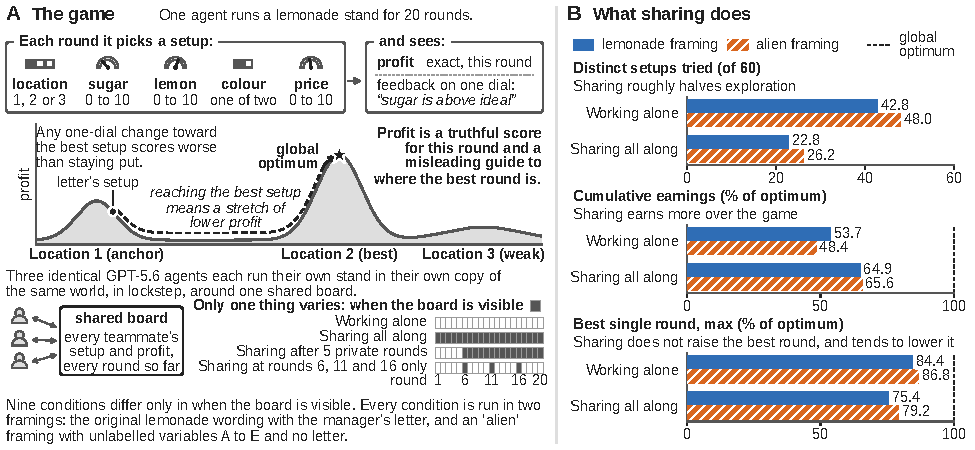
\includegraphics[width=\linewidth]{figures/fig_overview.pdf}
  \caption{\textbf{(A) The game.} An agent chooses a location and four settings each round and receives that round's profit and one line of feedback about one setting. Each location has a hidden ideal; the location the letter points to pays about half of the best one, and reaching the best one means scoring worse for a while. Three agents play the same world; conditions differ only in when the shared board of teammates' setups and profits is visible. \textbf{(B) What sharing does.} Sharing roughly halves the number of distinct setups a team tries, raises what the team earns over the game, and does not raise the best single round any teammate reaches. Means over eight worlds, GPT-5.6; blue is the lemonade framing, orange the alien framing.}
  \label{fig:overview}
\end{figure}

We put \NAgents{} identical GPT-5.6 agents in the same hidden world and vary one thing: when the shared board,
listing every teammate's setup and profit so far, is visible. Each agent is told to maximise the overall
performance of the business and nothing more. Nine conditions range from agents that never
see each other, through boards that open after two, five, ten or fifteen private rounds, to a board visible in
only three rounds, a board with an instruction to stay different from one's teammates, and agents that move
one at a time within each round. To check that the result is not an artefact of the lemonade wording and of
the recommended starting setup, every condition is also run in an alien framing, in which the same worlds are
described as five unlabelled decision variables with no recommendation. Each condition is run on
\NWorlds{} worlds, two or three times per world, so that we can report whether the first run's numbers
reproduce.

We show three things that hold in both framings. First, sharing collapses exploration
(Figure~\ref{fig:overview}B): a team that sees the
board from round one tries about half as many distinct setups as three agents working alone, and the later
the board opens, the more the team explores. This is the most reliable result in the paper: it holds in every
world, in every run and in both framings. Second, sharing raises cumulative earnings over the \NRounds{}
rounds in every sharing condition, because agents copy whoever is currently doing best and copying pays in
the current round. Third, sharing lowers the best single-round profit any teammate reaches. The size of the
drop is similar in the first run and in the repeats, but with \NWorlds{} worlds it is not statistically
reliable, and we say so. The sharing conditions that come closest to working alone on the best round are those
that preserve exploration: a board that opens late or in only three rounds, and the stay-different
instruction. Nothing we ran puts sharing reliably above working alone on the best round. A direct test of the
three-round board on sixteen further worlds puts it within a few points of working alone in both framings, and
a replication of three conditions on Claude
Opus 5.5 reproduces the exploration and earnings results, with the drop in the best round appearing in the
lemonade framing but not in the alien framing. A 60-round version of the two main conditions shows that the
trade is horizon-dependent in a way that turns on the letter: given time, sharing teams that start from a
common recommendation leave it and lose nothing on the best round while earning more, whereas teams with no
recommendation stay below working alone on the best round and keep a smaller earnings lead.

The contribution is a clean testbed and a measured answer. The testbed is small, deterministic, cheap to
run, and has a known global optimum in every world. This separates the two things a team might want: the
ceiling it reaches and the total it earns on the way. The answer is that for LLM agents on a landscape with a
valley, visibility trades the ceiling for the total, the mechanism is reduced search, and the lever that
restores the ceiling is limiting how often or how closely the agents look at each other. Section~\ref{sec:related}
places the study, Section~\ref{sec:method} describes the game, the framings, the conditions and the
measures, Section~\ref{sec:results} reports the results and their reproducibility, and
Section~\ref{sec:discussion} states what we think is established, what is not, and what we plan next.

\section{Related Work}\label{sec:related}

\paragraph{Exploration and exploitation in groups.}
\citet{march1991exploration} modelled an organisation whose members learn from a shared code and showed that
faster mutual learning raises average knowledge early and lowers it in the long run, because the code absorbs
the members' beliefs before the best belief has been found. \citet{lazer2007network} placed agents on an NK
landscape \citep{levinthal1997adaptation} and varied how densely they were connected: dense networks spread the
current best solution quickly, which raises short-run performance and lowers the long-run outcome, while
sparse networks keep diversity alive long enough to find better regions. \citet{fang2010balancing} found that
semi-isolated subgroups that occasionally exchange information outperform both fully connected and fully
isolated groups. Experiments with people reproduce the pattern. \citet{mason2012collaborative} let networked
participants search a landscape with a hidden peak and found that efficient networks did better on average
but could converge prematurely, and \citet{derex2016partial} found that partially connected groups accumulated
more cultural innovation than fully connected ones. Our periodic-board condition and our private-rounds
ladder are direct analogues of the sparse and semi-isolated structures in this literature, run with LLM agents
instead of simulated or human ones.

\paragraph{Search on rugged landscapes with people.}
\citet{ederer2013pay} designed the lemonade-stand game to test whether paying for early performance deters
exploration of a strategy that is better in the long run but worse at first. Participants who were paid every
period stayed near the recommended setup; participants whose early failures were tolerated explored more and
more often found the better location. \citet{billinger2014search} ran a related experiment on NK landscapes
and found that people search less than the landscape warrants, especially after early success. We keep the
game, the valley and the letter, and change the question from how the individual is paid to what the
individual can see of others.

\paragraph{LLM agents and exploration.}
Frozen LLMs explore poorly in bandit problems: they fail to return to the best arm, or play nearly uniformly,
except under engineered prompts \citep{krishnamurthy2024explore}, and their failures are greedy
\citep{schmied2025greedy}. Their exploration is also shaped by what the arms are called:
\citet{austin2026semantic} vary the labels of a bandit and find that semantic priors bias which arms are
tried. Our alien framing follows that idea. It keeps every number in the world and changes only the words,
so that any difference between framings is attributable to the labels and to the recommended starting setup,
not to the landscape.

\paragraph{Communication between LLM agents.}
Generative-agent systems let LLM agents observe and talk to one another \citep{park2023generative}, and
\citet{park2026scaling} study the minimal case we start from: identical agents, one shared workspace, no roles
and no orchestrator. They find that sharing beats the best of $k$ independent agents when a verifier ranks
partial progress correctly and that the advantage disappears when it cannot. Our world is the case they leave
open: a verifier that is correct about the current round and misleading about the direction of the best one.

\section{Methodology}\label{sec:method}

\subsection{The game}\label{sec:game}

One agent runs a stand for \NRounds{} rounds. Each round it chooses one of three locations, a sugar level, a
lemon level, one of two colours, and a price. Sugar, lemon and price run from 0.0 to 10.0 in steps of 0.1. The
agent then receives that round's profit and one line of customer feedback. Profit is deterministic. Each
location in a world has a hidden ideal setup and a hidden ceiling, and the profit for a setup is the
ceiling minus a linear penalty for every unit of distance from the ideal on each of sugar, lemon and price,
minus a flat penalty if the colour is wrong, floored at zero. The same setup in the same world always pays
the same profit. The feedback line picks one of sugar, lemon or price at random and says whether it is above,
below or at the ideal for the location the agent sold at. It is a local signal about one dial at one
location. It says nothing about other locations and never mentions colour. The agent never sees the profit
rule or the ideals; it has to find a good setup by trying things. Appendix~\ref{app:prompts} gives the
prompts verbatim.

\subsection{Worlds}\label{sec:worlds}

A world is a set of hidden ideals, one per location, together with each location's ceiling and penalty
slopes. Worlds are drawn by a generator that reproduces the structure of the original game
\citep{ederer2013pay}: one \emph{anchor} location with a ceiling between 90 and 110 and steep penalties, one
\emph{best} location with a ceiling between 180 and 220, equally steep penalties and a large colour penalty,
and a third location with a low ceiling and gentle penalties. A generated world is kept only if moving to the
best location without also changing the recipe pays less than staying at the anchor, so that reaching the top
requires a coordinated change of several variables and passes through a valley. The eight worlds used here
are the first eight of the validation split of the generator; no test world is used. Their global optima, the
most any setup can pay in one round, are listed in Appendix~\ref{app:worlds}. All scores below are expressed
as a share of the world's global optimum so that worlds can be compared. No setup outside the best location
pays more than 56.3\% of the optimum in any of the eight worlds.

\subsection{Two framings}\label{sec:framings}

\paragraph{Lemonade framing.}
The agent is told it runs a lemonade stand. Locations have their real names, such as school or stadium, and
the choices are called sugar, lemon, colour and price. The agent also receives a letter from the previous
manager describing the setup that worked for him at one location, with its profit, and saying that he never
tried another location and that other locations may need a very different recipe. The letter's setup is near,
but not at, the anchor location's ideal, and the anchor location is never the best one.

\paragraph{Alien framing.}
The worlds and their numbers are identical. Everything else is stripped away. The agent is told it runs a
business with five decision variables, A to E. Variable A takes the values A1, A2 and A3, which are the three
locations; B, C and E are sugar, lemon and price; D takes the values D1 and D2, the two colours. Profit is
called payoff. There is no letter and no recommended starting setup. Feedback has the same content as in the
lemonade framing, phrased as ``at this value of A, B is higher than ideal''. The alien framing was designed
following \citet{billinger2014search} and the label manipulation of \citet{austin2026semantic}: keep the
landscape, change only the words a language model has priors about.

\subsection{Teams and the shared board}\label{sec:board}

A team is \NAgents{} agents of the same model in the same world. Each agent runs its own stand in its own copy
of the world, so profits are not coupled and every number stays comparable with a single agent. Rounds are in
lockstep. When sharing is on, a shared board is appended to each agent's prompt listing, for every teammate and
every round so far, the setup chosen and the profit earned. In the default conditions all three agents choose
simultaneously from the board as it stood at the end of the previous round. Results are posted to the board
from round one in every condition, so a board that opens late already carries the private history. The
agents are not told how they are scored. The task instruction in every condition is ``Your goal is to
maximise the overall performance of the business'' (or ``of the lemonade stand''). Two details of the board's
wording are disclosed in Section~\ref{sec:limitations}.

\subsection{Conditions}\label{sec:conditions}

Nine conditions were run. They differ only in when the board is visible and, in one case, in what the agents
are told about it. Everything else is identical.

\begin{table}[H]
  \centering
  \caption{The nine conditions. Each was run in both framings on the same eight worlds.}
  \label{tab:conditions}
  \small
  \renewcommand{\arraystretch}{1.35}
  \begin{tabular}{p{4.6cm} p{10.2cm}}
    \toprule
    Condition & What happens \\
    \midrule
    Working alone & No shared board. Three agents play the same world without seeing each other. \\
    Sharing all along & The board is visible from round 1. \\
    Sharing after 2 private rounds & The board opens in round 3. \\
    Sharing after 5 private rounds & The board opens in round 6. \\
    Sharing after 10 private rounds & The board opens in round 11. \\
    Sharing after 15 private rounds & The board opens in round 16. \\
    Sharing at rounds 6, 11 and 16 only & The board is visible only in those three rounds, five rounds apart, and private otherwise. We call this the periodic board. \\
    Sharing, told to stay different & The board is visible from round 1. Each agent is also told to pick an approach different from the ones already claimed, to adopt a teammate's approach only when its posted result is clearly better, and to keep one variation of its own when it does. \\
    One agent at a time & The board is visible from round 1. Within each round the agents move in a rotating order (1-2-3, then 2-3-1, then 3-1-2), so the second mover sees the first mover's result from the current round and the third sees both. \\
    \bottomrule
  \end{tabular}
\end{table}

Working alone is the reference. Three agents working alone receive the same \NAttempts{} attempts in a world
as a sharing team, so the two are scored on the same number of tries. Where the text says the periodic board it
means the condition in which the board is visible only at rounds 6, 11 and 16.

\subsection{Measures}\label{sec:measures}

All measures are computed per team per world and expressed as a share of the world's global optimum, except
the count of distinct setups.

\begin{itemize}[leftmargin=*, itemsep=2pt]
  \item \textbf{Maximum single-round profit (max):} the highest profit any one agent on the team reached in
    any round, as a share of the global optimum. For working alone this is the best of the three independent
    agents, so both arms are scored on the best of \NAttempts{} attempts. This measures whether the team
    found the best setup.
  \item \textbf{Cumulative earnings:} everything the three agents earned over all \NRounds{} rounds, as a
    share of what they would have earned by hitting the best setup in every round. This measures what the
    team earned while it was still searching.
  \item \textbf{Distinct setups:} the number of different full setups (location, sugar, lemon, colour, price)
    among the team's \NAttempts{} attempts, pooled across the three agents. This measures how much the team
    explored.
  \item \textbf{Reached the best location:} whether the team's max exceeds 60\% of the optimum, which only
    a setup at the best location can do.
\end{itemize}

The first two measures are the two goals a team might have, best-arm identification and regret minimisation,
and the agents are instructed on neither.

\subsection{Model, runs and statistics}\label{sec:stats}

The main runs use GPT-5.6 (gpt-5.6-sol) through the OpenAI API with the provider's default sampling. Each
condition was run on the eight worlds in both framings. Three follow-ups, each planned before it was run, are
reported in Section~\ref{sec:results}: working alone and the periodic board on sixteen further worlds in both
framings, three conditions on a second model, Claude Opus 5.5, and working alone and sharing all along in
60-round games on the eight worlds. The first run of every condition was made in October 2026. To
test whether the first run's numbers were a fluke, every condition was then repeated under a plan written
before any repeat was run: working alone, sharing all along and sharing at rounds 6, 11 and 16 were repeated
twice more, giving three runs per world, and the other six conditions were repeated once, giving two runs per
world, in both framings. Repeats use their own environment seeds for the customer-feedback draws. Every planned
episode completed, and no run was stopped, extended or excluded on the basis of its result.

The unit of analysis is the world. A world's value for a condition is the mean over its runs. Condition means
in the tables are the mean over the eight worlds of those values, and the figure after $\pm$ is the sample
standard deviation of the condition's run means across runs, which shows the run-to-run wobble. For each
contrast we take the paired difference between a sharing condition and working alone within each world, and
report the mean, a 95\% $t$ interval over the eight world-level differences, and the exact two-sided sign-flip
permutation test over the eight worlds. The smallest $p$ this test can produce with eight worlds is
$0.0078$. The headline contrast is the mean of the eight sharing conditions minus working alone, reported
for the first run alone, for the repeat runs alone and for all runs, so that the reader can see whether the
first run and the repeats agree.

\section{Results}\label{sec:results}

\paragraph{Overview.}
Table~\ref{tab:main} gives every condition's mean on the three measures in both framings, averaged over runs,
with the standard deviation across runs. Table~\ref{tab:contrasts} gives the headline contrast, the mean of the
eight sharing conditions relative to working alone, with its interval and test, separately for the first run, the
repeat runs and all runs. Three patterns appear in both framings: sharing cuts the number of distinct setups,
raises cumulative earnings and lowers the max. The first two are statistically reliable with eight worlds.
The third is consistent in sign and size across runs but is not. We report them in that order because the
first is the mechanism we think produces the other two.

\begin{table}[t]
  \centering
  \caption{Condition means over the eight worlds, averaged over runs, $\pm$ standard deviation across runs. Max and cumulative earnings are shares of the world's global optimum in percent; distinct setups are counts out of \NAttempts{} attempts.}
  \label{tab:main}
  \small
  \setlength{\tabcolsep}{4pt}
  \begin{tabular}{l c ccc ccc}
\toprule
 & & \multicolumn{3}{c}{Lemonade framing} & \multicolumn{3}{c}{Alien framing} \\
\cmidrule(lr){3-5} \cmidrule(lr){6-8}
Condition & Runs & Max & Cumulative & Distinct & Max & Cumulative & Distinct \\
\midrule
Working alone & 3 & 84.4 $\pm$ 4.0 & 53.7 $\pm$ 2.8 & 42.8 $\pm$ 2.1 & 86.8 $\pm$ 4.1 & 48.4 $\pm$ 2.5 & 48.0 $\pm$ 1.2 \\
Sharing all along & 3 & 75.4 $\pm$ 0.9 & 64.9 $\pm$ 3.0 & 22.8 $\pm$ 1.1 & 71.2 $\pm$ 7.5 & 58.8 $\pm$ 7.2 & 25.1 $\pm$ 0.4 \\
Sharing after 2 private rounds & 2 & 69.0 $\pm$ 0.4 & 58.9 $\pm$ 1.1 & 21.9 $\pm$ 0.3 & 76.8 $\pm$ 0.4 & 60.7 $\pm$ 2.6 & 26.1 $\pm$ 0.3 \\
Sharing after 5 private rounds & 2 & 70.0 $\pm$ 8.0 & 58.9 $\pm$ 4.6 & 26.4 $\pm$ 2.6 & 74.8 $\pm$ 14.1 & 56.7 $\pm$ 8.1 & 28.6 $\pm$ 0.4 \\
Sharing after 10 private rounds & 2 & 72.7 $\pm$ 4.6 & 58.8 $\pm$ 2.9 & 31.9 $\pm$ 2.2 & 83.6 $\pm$ 3.8 & 57.2 $\pm$ 3.7 & 36.6 $\pm$ 0.9 \\
Sharing after 15 private rounds & 2 & 81.5 $\pm$ 7.7 & 57.1 $\pm$ 3.3 & 39.6 $\pm$ 3.4 & 84.5 $\pm$ 3.7 & 53.0 $\pm$ 2.6 & 42.9 $\pm$ 1.3 \\
Sharing at rounds 6, 11 and 16 only & 3 & 78.8 $\pm$ 3.5 & 60.9 $\pm$ 0.9 & 37.1 $\pm$ 2.2 & 89.7 $\pm$ 4.5 & 59.9 $\pm$ 4.4 & 42.8 $\pm$ 2.4 \\
Sharing, told to stay different & 2 & 78.5 $\pm$ 4.1 & 67.3 $\pm$ 6.1 & 41.4 $\pm$ 0.1 & 88.3 $\pm$ 5.0 & 67.3 $\pm$ 3.4 & 45.4 $\pm$ 1.5 \\
One agent at a time & 2 & 81.2 $\pm$ 0.4 & 72.1 $\pm$ 2.9 & 18.4 $\pm$ 1.1 & 72.4 $\pm$ 14.4 & 61.9 $\pm$ 9.2 & 21.1 $\pm$ 1.1 \\
\bottomrule
\end{tabular}
  \figurenote{Runs is the number of runs per world. The per-world values behind each mean are in Appendix~\ref{app:perworld}.}
\end{table}

\begin{table}[t]
  \centering
  \caption{Mean of the eight sharing conditions relative to working alone, paired within worlds. 95\% $t$ intervals over the eight world-level differences and exact sign-flip $p$-values. Max and cumulative earnings in percentage points of the optimum; distinct setups in counts.}
  \label{tab:contrasts}
  \scriptsize
  \setlength{\tabcolsep}{3.5pt}
  \begin{tabular}{l l rc rc rc}
\toprule
 & & \multicolumn{2}{c}{First run} & \multicolumn{2}{c}{Repeat runs only} & \multicolumn{2}{c}{All runs} \\
\cmidrule(lr){3-4} \cmidrule(lr){5-6} \cmidrule(lr){7-8}
Measure & Framing & Difference [95\% CI] & $p$ & Difference [95\% CI] & $p$ & Difference [95\% CI] & $p$ \\
\midrule
Max & lemonade & -8.6 [-24.7, +7.6] & 0.273 & -7.4 [-22.6, +7.7] & 0.312 & -8.5 [-21.9, +4.8] & 0.219 \\
 & alien & -5.1 [-28.3, +18.1] & 0.656 & -8.4 [-23.4, +6.5] & 0.234 & -6.6 [-17.6, +4.4] & 0.227 \\
 & both & -6.8 [-22.5, +8.8] & 0.312 & -7.9 [-17.9, +2.0] & 0.062 & -7.6 [-17.9, +2.7] & 0.109 \\
\addlinespace
Cumulative & lemonade & +10.1 [+4.2, +16.0] & 0.008 & +8.6 [+1.8, +15.3] & 0.031 & +8.7 [+4.1, +13.2] & 0.016 \\
 & alien & +15.0 [+4.7, +25.4] & 0.031 & +8.2 [+2.1, +14.4] & 0.023 & +11.0 [+7.7, +14.3] & 0.008 \\
 & both & +12.6 [+9.1, +16.0] & 0.008 & +8.4 [+3.3, +13.5] & 0.016 & +9.8 [+6.9, +12.7] & 0.008 \\
\addlinespace
Distinct setups & lemonade & -11.9 [-18.9, -5.0] & 0.008 & -13.0 [-17.5, -8.4] & 0.008 & -12.9 [-17.6, -8.2] & 0.008 \\
 & alien & -13.2 [-18.6, -7.8] & 0.008 & -15.3 [-19.1, -11.4] & 0.008 & -14.5 [-17.2, -11.7] & 0.008 \\
 & both & -12.6 [-16.8, -8.4] & 0.008 & -14.1 [-16.7, -11.5] & 0.008 & -13.7 [-16.2, -11.2] & 0.008 \\
\bottomrule
\end{tabular}
  \figurenote{``Both'' averages the two framings within each world before taking the difference. The smallest attainable $p$ with eight worlds is 0.0078.}
\end{table}

\paragraph{Sharing cuts exploration in half.}
This is the most reliable result in the paper and, we think, the mechanism behind the other two. Three agents
working alone try \LemSoloUniq{} distinct setups out of \NAttempts{} in the lemonade framing and
\AliSoloUniq{} in the alien framing. A team that shares from round 1 tries \LemShareUniq{} and
\AliShareUniq{}. Averaged over all sharing conditions the drop is \AllLemUniq{} setups in the lemonade
framing and \AllAliUniq{} in the alien framing, with $p=\AllLemUniqP$ in both, and the sign is the same in
all eight worlds, in every run and in both framings. The later the board opens, the more the team explores
(Table~\ref{tab:main}). Opening the board in only three rounds, or adding the stay-different instruction,
keeps exploration close to the working-alone level. One agent at a time explores least of all. The drop is
not only in recipes: once the board is open, the three agents choose the same location in about
\SameLocShareLem\% of agent-rounds in the lemonade framing and \SameLocShareAli\% in the alien framing,
against \SameLocSoloLem\% and \SameLocSoloAli\% for agents working alone.

\paragraph{Sharing raises cumulative earnings.}
Working alone earns the least in both framings: \LemSoloSum\% of the ceiling in the lemonade framing and
\AliSoloSum\% in the alien framing. Every sharing condition earns more. Averaged over the sharing conditions
the gain is \AllLemSum{} points ($p=\AllLemSumP$) and \AllAliSum{} points ($p=\AllAliSumP$), and
\AllBothSum{} points with the framings pooled ($p=\AllBothSumP$). One agent at a time earns the most in the
lemonade framing (\LemStaggerSum\%) and the stay-different instruction earns the most in the alien framing
(\AliProtocolSum\%). The reason is visible in the board traces: once agents can see each other, they copy
whoever is doing best so far, and copying a good setup pays in the current round. Each agent's own best round
is also higher under sharing, by \OwnBestLem{} points in the lemonade framing and \OwnBestAli{} in the alien
framing, so sharing makes the typical agent better off even as it makes the team's ceiling lower.

\paragraph{Sharing lowers the max, but not reliably.}
In the lemonade framing working alone has the highest max, \LemSoloMax\%, and every sharing condition is
below it, by about 3 to 15 points; sharing all along is at \LemShareMax\%. In the alien framing working alone
is at \AliSoloMax\% and sharing all along at \AliShareMax\%. The pooled drop is \AllLemMax{} points in the
lemonade framing [\AllLemMaxLo, \AllLemMaxHi], \AllAliMax{} in the alien framing [\AllAliMaxLo,
\AllAliMaxHi] and \AllBothMax{} with the framings pooled [\AllBothMaxLo, \AllBothMaxHi], with $p$ between
\AllBothMaxP{} and \AllAliMaxP. The size of the drop in the repeats is about the same as in the first run
(Table~\ref{tab:contrasts}), so the effect reproduced, but with eight worlds the interval includes zero and
we do not claim it as established. The max is a best-of-\NAttempts{} measure, so a world's value moves by
tens of points depending on whether any one of the sixty attempts landed at the best location, which is why it
is so much noisier than the other two measures. Table~\ref{tab:reached} counts, for each condition, the
world-runs in which the team reached the best location at all: working alone did so in \LemSoloReached{}
world-runs in the lemonade framing and \AliSoloReached{} in the alien framing; sharing all along did so in
\LemShareReached{} and \AliShareReached{} respectively, the same share in both framings.

\begin{table}[t]
  \centering
  \caption{World-runs in which the team's best round was at the best location (max above 60\% of the optimum), out of the world-runs played.}
  \label{tab:reached}
  \small
  \begin{tabular}{l cc cc}
\toprule
 & \multicolumn{2}{c}{Lemonade framing} & \multicolumn{2}{c}{Alien framing} \\
\cmidrule(lr){2-3} \cmidrule(lr){4-5}
Condition & World-runs & Share & World-runs & Share \\
\midrule
Working alone & 17 of 24 & 71\% & 19 of 24 & 79\% \\
Sharing all along & 12 of 24 & 50\% & 16 of 24 & 67\% \\
Sharing after 2 private rounds & 6 of 16 & 38\% & 8 of 16 & 50\% \\
Sharing after 5 private rounds & 6 of 16 & 38\% & 13 of 16 & 81\% \\
Sharing after 10 private rounds & 7 of 16 & 44\% & 11 of 16 & 69\% \\
Sharing after 15 private rounds & 10 of 16 & 62\% & 14 of 16 & 88\% \\
Sharing at rounds 6, 11 and 16 only & 14 of 24 & 58\% & 17 of 24 & 71\% \\
Sharing, told to stay different & 9 of 16 & 56\% & 12 of 16 & 75\% \\
One agent at a time & 10 of 16 & 62\% & 7 of 16 & 44\% \\
\bottomrule
\end{tabular}
\end{table}

\paragraph{Timing of the board.}
Figure~\ref{fig:timing} plots the max against the round in which the board opens. The two framings differ in
shape. In the lemonade framing the worst time to open the board is the middle of the game: sharing after 2 or
5 private rounds is the lowest, and opening it very late recovers most of the loss. In the alien framing the
worst time is the start, and the curve climbs as the board opens later, coming within about 3 points of working
alone at rounds 11 and 16. Neither curve reaches its working-alone line. We think the letter is the most
likely reason for the different shapes: in the lemonade framing all three agents start near the letter's
location, so a board that opens in the middle shows them three versions of the same wrong answer at the moment
they would otherwise start to leave it. In the alien framing there is no common starting point, and private
rounds let the agents spread out before the board consolidates them. This has not been tested directly; the
controls that would test it are described in Section~\ref{sec:next}.

\begin{figure}[t]
  \centering
  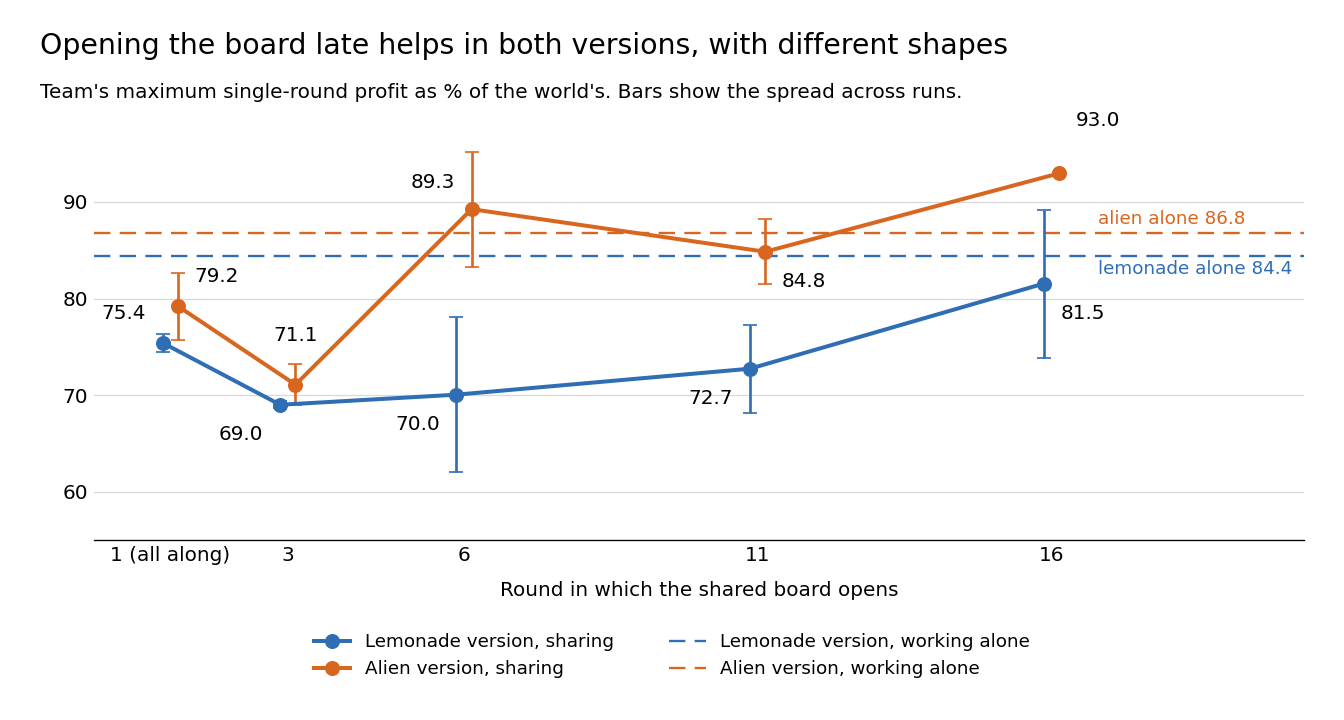
\includegraphics[width=0.78\linewidth]{figures/fig_sharing_timing_runs.png}
  \caption{Team max as a share of the world's optimum, by the round in which the shared board opens.}
  \label{fig:timing}
  \figurenote{Blue is the lemonade framing and orange the alien framing. The dashed line in each colour is the working-alone level for that framing. GPT-5.6, eight worlds, two or three runs per world; bars show the standard deviation across runs.}
\end{figure}

\paragraph{Per-condition contrasts.}
Table~\ref{tab:percondition} gives each sharing condition's difference from working alone on every measure. On the max, no
sharing condition is above working alone in the lemonade framing. In the alien framing two are slightly above
it: sharing at rounds 6, 11 and 16 only, at \AliPeriodicMax\% against \AliSoloMax\% (difference
\AliPeriodicDiff{} points [\AliPeriodicLo, \AliPeriodicHi], $p=\AliPeriodicP$), and the stay-different
instruction, at \AliProtocolMax\% (\AliProtocolDiff{} points, $p=\AliProtocolP$). Neither is distinguishable
from working alone. The first gap comes down to one extra world-run in which the team reached the best
location, \AliPeriodicReached{} against \AliSoloReached{} for working alone; the condition was ahead of
working alone in two of its three runs and behind in the third, and in the lemonade framing the same condition
is \LemPeriodicMax\% against \LemSoloMax\%, below working alone. We therefore read both as level with working
alone, not better. What the two have in common is that they are the two sharing designs that keep exploration
near the working-alone level.

\paragraph{Replication on sixteen further worlds.}
Because the test over eight worlds cannot separate a gap of a few points from zero, we ran the periodic-board
condition and working alone on sixteen further worlds that no condition had touched, three runs per world, in
both framings, with the analysis fixed before each run. Table~\ref{tab:worlds24} gives the paired differences
on the new worlds, on the pilot worlds and on all 24. The pre-specified primary result, in both framings, is
that the periodic board is level with working alone on the max. In the lemonade framing it is \WLAllMax{}
points relative to working alone over all 24 worlds [\WLAllMaxLo, \WLAllMaxHi], $p\WLAllMaxP$, with
\WLAllMaxUp{} worlds up and \WLAllMaxDown{} down; the \WLPilotMax{}-point deficit on the pilot worlds did not
reproduce on the new ones (\WLNewMax{} points). In the alien framing it is \WAllMax{} points [\WAllMaxLo,
\WAllMaxHi], $p\WAllMaxP$, and the small advantage seen on the pilot worlds did not reproduce either
(\WNewMax{} points on the new worlds); both arms reached the best location in the same share of world-runs,
\WAllReachedArm\% against \WAllReachedSolo\%. The other two effects reproduced in both framings and are now
reliable on 24 worlds: cumulative earnings \WLAllSum{} points [\WLAllSumLo, \WLAllSumHi] in the lemonade
framing and \WAllSum{} [\WAllSumLo, \WAllSumHi] in the alien framing, both $p\WAllSumP$; distinct setups
\WLAllUniq{} [\WLAllUniqLo, \WLAllUniqHi] and \WAllUniq{} [\WAllUniqLo, \WAllUniqHi], both $p\WAllUniqP$, with
the count lower in \WLAllUniqDown{} and \WAllUniqDown{} of the \WAllUniqN{} worlds.

\begin{table}[t]
  \centering
  \caption{Sharing at rounds 6, 11 and 16 relative to working alone, paired over worlds, both framings. Three runs per world. Max and cumulative earnings in percentage points of the optimum; distinct setups in counts; reached best location in percentage points of world-runs.}
  \label{tab:worlds24}
  \scriptsize
  \setlength{\tabcolsep}{3.5pt}
  \begin{tabular}{l l rc rc rc}
\toprule
 & & \multicolumn{2}{c}{16 new worlds} & \multicolumn{2}{c}{8 pilot worlds} & \multicolumn{2}{c}{All 24 worlds} \\
\cmidrule(lr){3-4} \cmidrule(lr){5-6} \cmidrule(lr){7-8}
Framing & Measure & Difference [95\% CI] & $p$ & Difference [95\% CI] & $p$ & Difference [95\% CI] & $p$ \\
\midrule
Lemonade & Max & +0.8 [-6.9, +8.5] & 0.828 & -5.6 [-21.7, +10.5] & 0.438 & -1.3 [-8.1, +5.4] & 0.684 \\
 & Cumulative & +10.4 [+6.3, +14.5] & $<$0.001 & +7.2 [+0.5, +13.9] & 0.023 & +9.3 [+6.0, +12.6] & $<$0.001 \\
 & Distinct setups & -6.9 [-9.7, -4.1] & $<$0.001 & -5.8 [-9.2, -2.3] & 0.031 & -6.5 [-8.5, -4.5] & $<$0.001 \\
 & Reached best location (\%) & -0.0 [-15.9, +15.9] & 1.000 & -12.5 [-42.1, +17.1] & 0.531 & -4.2 [-17.5, +9.2] & 0.668 \\
\addlinespace
Alien & Max & -0.6 [-4.8, +3.5] & 0.875 & +2.9 [-12.7, +18.5] & 0.703 & +0.6 [-4.6, +5.7] & 0.838 \\
 & Cumulative & +5.9 [+2.5, +9.4] & 0.002 & +11.5 [+4.9, +18.1] & 0.016 & +7.8 [+4.7, +10.9] & $<$0.001 \\
 & Distinct setups & -7.5 [-9.2, -5.8] & $<$0.001 & -5.2 [-8.6, -1.9] & 0.023 & -6.7 [-8.2, -5.2] & $<$0.001 \\
 & Reached best location (\%) & -2.1 [-12.3, +8.1] & 1.000 & +4.2 [-23.5, +31.8] & 1.000 & -0.0 [-10.2, +10.2] & 1.000 \\
\bottomrule
\end{tabular}
  \figurenote{The sixteen new worlds are not the pilot worlds' equals in level: in the alien framing they are easier for both arms (working alone reaches a max of \WNewMaxSolo\% against \AliSoloMax\%) and in the lemonade framing harder (\WLNewMaxSolo\% against \LemSoloMax\%), so levels are not comparable across the two sets; the paired differences are. The same sixteen worlds are used in both framings.}
\end{table}

\begin{table}[t]
  \centering
  \caption{Each sharing condition's difference from working alone, paired within worlds, all runs. Max and cumulative earnings in percentage points; distinct setups in counts. $^{\ast}$ marks $p<0.05$ on the exact sign-flip test.}
  \label{tab:percondition}
  \small
  \setlength{\tabcolsep}{4pt}
  \begin{tabular}{l ccc ccc}
\toprule
 & \multicolumn{3}{c}{Lemonade framing} & \multicolumn{3}{c}{Alien framing} \\
\cmidrule(lr){2-4} \cmidrule(lr){5-7}
Difference from working alone & Max & Cumulative & Distinct & Max & Cumulative & Distinct \\
\midrule
Sharing all along & -9.0 & +11.2$^{\ast}$ & -20.1$^{\ast}$ & -15.6 & +10.4 & -23.0$^{\ast}$ \\
Sharing after 2 private rounds & -15.4 & +5.1 & -20.9$^{\ast}$ & -10.0 & +12.2 & -22.0$^{\ast}$ \\
Sharing after 5 private rounds & -14.4 & +5.2 & -16.4$^{\ast}$ & -12.0 & +8.3 & -19.4$^{\ast}$ \\
Sharing after 10 private rounds & -11.7 & +5.1 & -10.9$^{\ast}$ & -3.2 & +8.8$^{\ast}$ & -11.4$^{\ast}$ \\
Sharing after 15 private rounds & -2.9 & +3.4 & -3.3 & -2.3 & +4.6 & -5.1$^{\ast}$ \\
Sharing at rounds 6, 11 and 16 only & -5.6 & +7.2$^{\ast}$ & -5.7$^{\ast}$ & +2.9 & +11.5$^{\ast}$ & -5.2$^{\ast}$ \\
Sharing, told to stay different & -5.9 & +13.6 & -1.4 & +1.5 & +18.9$^{\ast}$ & -2.6 \\
One agent at a time & -3.2 & +18.4$^{\ast}$ & -24.4$^{\ast}$ & -14.4 & +13.4 & -26.9$^{\ast}$ \\
\bottomrule
\end{tabular}
\end{table}

\paragraph{Replication on a second model.}
To check that the pattern is not specific to GPT-5.6, we ran working alone, sharing all along and sharing at
rounds 6, 11 and 16 on Claude Opus 5.5, in both framings, on the eight pilot worlds, two runs per world, with
the analysis fixed before the runs. Table~\ref{tab:claude} puts the paired
differences beside GPT-5.6's on the same worlds. The drop in exploration reproduces in every cell: sharing all
along cuts distinct setups by \CLemUniqShare{} in the lemonade framing and \CAliUniqShare{} in the alien
framing, both $p\CLemUniqShareP$, and the periodic board by less. Cumulative earnings are higher under sharing
in all four cells, reliably so for sharing all along in the alien framing (\CAliSumShare{} points,
$p\CAliSumShareP$). On the max the two models differ in one place. For Claude, sharing all along lowers the max
in the lemonade framing by \CLemMaxShare{} points [\CLemMaxShareLo, \CLemMaxShareHi], a larger drop than
GPT-5.6's, with the team reaching the best location in \CLemReachedShareArm\% of world-runs against
\CLemReachedShareSolo\% working alone; in the alien framing it is level with working alone (\CAliMaxShare{}
points), where GPT-5.6 showed a drop. The periodic board is level with working alone on the max in both
framings for Claude (\CLemMaxPeriodic{} and \CAliMaxPeriodic{} points), as it is for GPT-5.6 on 24 worlds.
Claude working alone also reaches a higher max than GPT-5.6 in the lemonade framing (\CLemMaxShareSolo\%
against \LemSoloMax\%), so the two models search differently; what they share is that visibility reduces
search, raises earnings, and never raises the ceiling.

\begin{table}[t]
  \centering
  \caption{Second model. Each sharing condition's difference from working alone, paired over the eight pilot worlds, for Claude Opus 5.5 (two runs per world) and GPT-5.6 (two or three runs per world) on the same worlds. Max and cumulative earnings in percentage points of the optimum; distinct setups in counts. $^{\ast}$ marks $p<0.05$ on the exact sign-flip test.}
  \label{tab:claude}
  \scriptsize
  \setlength{\tabcolsep}{3pt}
  \begin{tabular}{l l cc cc}
\toprule
 & & \multicolumn{2}{c}{Claude Opus 5.5} & \multicolumn{2}{c}{GPT-5.6} \\
\cmidrule(lr){3-4} \cmidrule(lr){5-6}
Framing & Measure & Sharing all along & Sharing at 6, 11, 16 & Sharing all along & Sharing at 6, 11, 16 \\
\midrule
Lemonade & Max & -14.9 [-29.3, -0.6] & -3.1 [-11.0, +4.9] & -9.0 [-25.3, +7.2] & -5.6 [-21.7, +10.5] \\
 & Cumulative & +4.0 [-8.2, +16.3] & +7.0 [-1.8, +15.7] & +11.2$^{\ast}$ [+3.1, +19.4] & +7.2$^{\ast}$ [+0.5, +13.9] \\
 & Distinct setups & -18.8$^{\ast}$ [-21.5, -16.1] & -6.1$^{\ast}$ [-8.1, -4.0] & -20.1$^{\ast}$ [-26.9, -13.3] & -5.7$^{\ast}$ [-9.2, -2.3] \\
\addlinespace
Alien & Max & +3.0 [-10.1, +16.0] & -5.1 [-13.5, +3.2] & -7.6 [-30.9, +15.7] & -3.1 [-16.5, +10.2] \\
 & Cumulative & +7.5 [-2.0, +16.9] & +3.5 [-1.9, +8.9] & +17.2$^{\ast}$ [+3.5, +30.9] & +8.5$^{\ast}$ [+3.7, +13.3] \\
 & Distinct setups & -9.2$^{\ast}$ [-15.5, -2.9] & -1.6 [-5.4, +2.3] & -21.8$^{\ast}$ [-24.7, -18.9] & -5.6$^{\ast}$ [-9.6, -1.5] \\
\bottomrule
\end{tabular}
\end{table}

\paragraph{A longer horizon.}
Whether the trade between earning and finding is a property of the game or of stopping at round 20 can be
tested directly. We ran working alone and sharing all along for 60 rounds, in both
framings, on the eight pilot worlds, three runs per world, with the analysis and a decision rule fixed before
the runs. These are new games, not continuations: every prompt says ``Round $r$ of 60'', and an agent that
believed round 20 was the last played its last rounds accordingly. Table~\ref{tab:h60} gives the paired
differences over the whole 60-round game, over rounds 21 to 60 alone, and, for comparison, in the 20-round
game on the same worlds. The two framings move in opposite directions. With the letter, time favours sharing.
The drop in the max closes from \HLemMaxGame{} points in the 20-round game to \HLemMaxFull{} points
[\HLemMaxFullLo, \HLemMaxFullHi] over 60 rounds, as sharing teams eventually leave the recommended location
and reach the best one in \HLemReachedFullArm\% of world-runs against \HLemReachedFullSolo\% working alone,
while the cumulative lead of sharing grows to \HLemSumFull{} points [\HLemSumFullLo, \HLemSumFullHi]
($p\HLemSumFullP$, \HLemSumFullUp{} of 8 worlds) and is still \HLemSumLate{} points in rounds 21 to 60.
Without the letter, time favours the lone agents. The drop in the max does not close (\HAliMaxFull{} points
[\HAliMaxFullLo, \HAliMaxFullHi]; \HAliReachedFullArm\% of sharing world-runs reach the best location against
\HAliReachedFullSolo\% working alone), and the cumulative lead of sharing shrinks from \HAliSumGame{} points
in the 20-round game to \HAliSumFull{} points over 60 rounds [\HAliSumFullLo, \HAliSumFullHi], and is
\HAliSumLate{} points in rounds 21 to 60, with \HAliSumLateDown{} of 8 worlds favouring working alone. The
collapse of exploration is unchanged by the horizon: sharing cuts distinct setups by \HLemUniqFull{} and
\HAliUniqFull{} over 60 rounds, and in rounds 21 to 60 a sharing team tries \HLemUniqLateArm{} and
\HAliUniqLateArm{} distinct setups against \HLemUniqLateSolo{} and \HAliUniqLateSolo{} for three agents working
alone. Being told the game is longer also changes early play. In the first 20 rounds of the 60-round game,
sharing teams in the lemonade framing reach a max of \ELemShareMaxHsixty\% against \ELemShareMaxHtwenty\% in
the 20-round game (\ELemShareMax{} points, $p\ELemShareMaxP$), and lone agents in both framings try more
distinct setups early (\ELemSoloUniq{} and \EAliSoloUniq{}, $p\ELemSoloUniqP$ and $p\EAliSoloUniqP$).

\begin{table}[t]
  \centering
  \caption{A longer horizon. Sharing all along relative to working alone, paired over the eight pilot worlds, GPT-5.6, three runs per world, in 60-round games and, for comparison, in the 20-round game on the same worlds. Max and cumulative earnings in percentage points of the optimum; distinct setups in counts; reached best location in percentage points of world-runs. $^{\ast}$ marks $p<0.05$ on the exact sign-flip test.}
  \label{tab:h60}
  \scriptsize
  \setlength{\tabcolsep}{4pt}
  \begin{tabular}{l l c cc}
\toprule
 & & 20-round game & \multicolumn{2}{c}{60-round game} \\
\cmidrule(lr){3-3} \cmidrule(lr){4-5}
Framing & Measure & rounds 1--20 & rounds 1--60 & rounds 21--60 \\
\midrule
Lemonade & Max & -9.0 [-25.3, +7.2] & -1.4 [-9.8, +7.0] & -1.4 [-9.8, +7.0] \\
 & Cumulative & +11.2$^{\ast}$ [+3.1, +19.4] & +18.2$^{\ast}$ [+11.6, +24.8] & +14.8$^{\ast}$ [+6.8, +22.8] \\
 & Distinct setups & -20.1$^{\ast}$ [-26.9, -13.3] & -40.5$^{\ast}$ [-46.2, -34.8] & -14.5$^{\ast}$ [-21.7, -7.2] \\
 & Reached best location & -20.8 [-53.9, +12.3] & -4.2 [-22.0, +13.7] & -4.2 [-22.0, +13.7] \\
\addlinespace
Alien & Max & -15.6 [-35.9, +4.7] & -19.0 [-41.0, +2.9] & -19.0 [-41.0, +2.9] \\
 & Cumulative & +10.4 [-1.9, +22.7] & +2.2 [-15.7, +20.1] & -3.0 [-23.5, +17.5] \\
 & Distinct setups & -23.0$^{\ast}$ [-25.9, -20.0] & -33.5$^{\ast}$ [-41.4, -25.7] & -11.7$^{\ast}$ [-17.5, -5.9] \\
 & Reached best location & -29.2 [-63.9, +5.6] & -33.3 [-72.8, +6.1] & -33.3 [-72.8, +6.1] \\
\bottomrule
\end{tabular}
\end{table}

\paragraph{Reproducibility.}
Figure~\ref{fig:intervals} and Table~\ref{tab:contrasts} compare the first run with the repeats. The three
headline contrasts have the same sign in the first run, in the repeats and in all runs, in both framings. Per
condition, the repeats fall on the same side of working alone as the first run in \AgreeSame{} of \AgreeOf{}
condition-measure-framing cells, and the four exceptions are cells within 7 points or 3 setups of zero both
times (Appendix~\ref{app:agree}). The repeats did not change any conclusion of the first run. They narrowed the
intervals on cumulative earnings and distinct setups enough to make both reliable in each framing on its
own, and they left the max where it was: a consistent drop that eight worlds cannot separate from zero.

\begin{figure}[t]
  \centering
  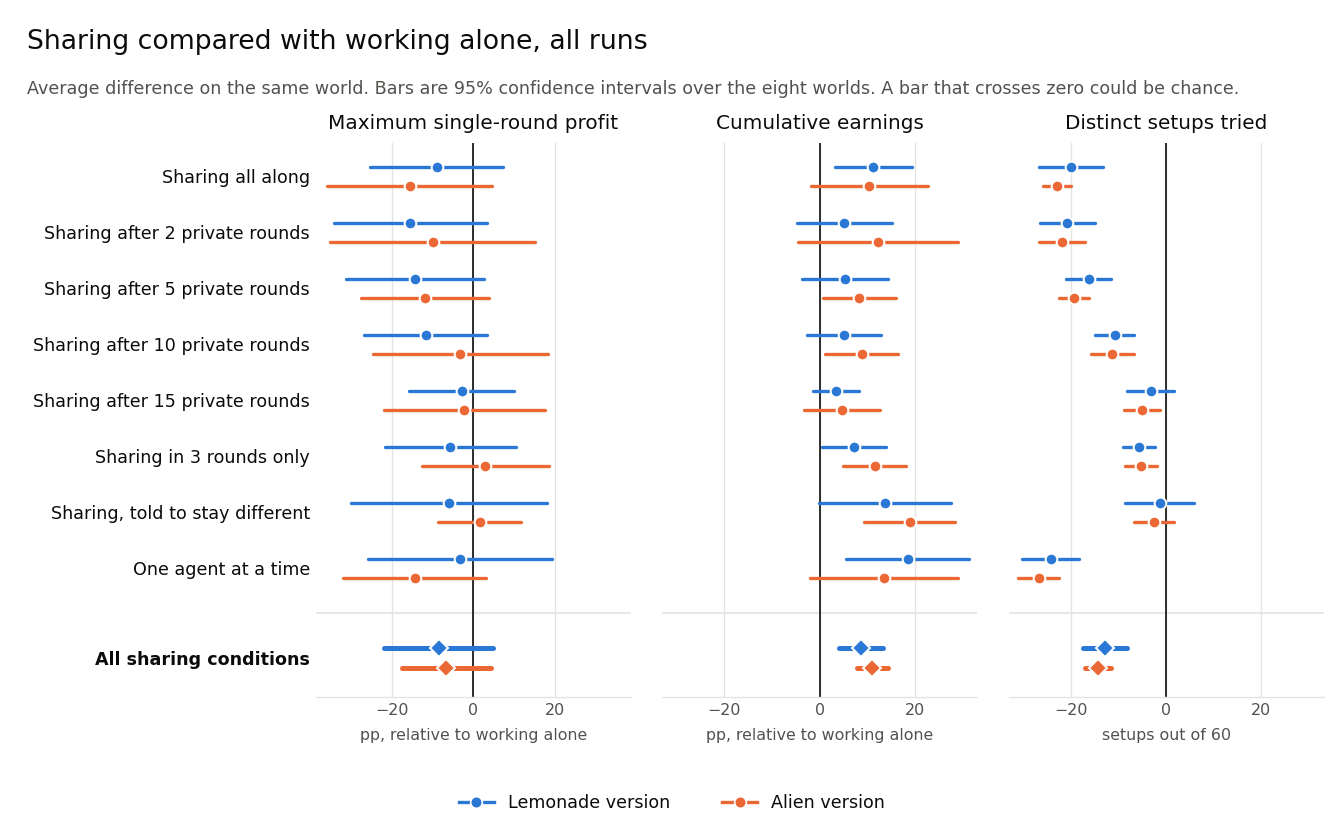
\includegraphics[width=0.95\linewidth]{figures/fig_sharing_intervals.png}
  \caption{Each sharing condition, and the mean of all sharing conditions, relative to working alone, with 95\% intervals, all runs.}
  \label{fig:intervals}
  \figurenote{Paired over the eight worlds; blue is the lemonade framing and orange the alien framing. For the pooled contrast in the bottom row, the intervals for cumulative earnings and distinct setups exclude zero in both framings and the interval for the max includes zero in both.}
\end{figure}

\section{Discussion}\label{sec:discussion}

\paragraph{The trade.}
Looked at together, the results describe a trade between earning more along the way and finding less at the
end. Sharing raises what the team earns while it looks and lowers what the team eventually finds. A team that
cares about the ceiling seems to do better keeping its agents apart for a while. A team that cares about the
total seems to do better letting them copy each other. The 60-round runs show that this trade is a horizon
effect, and that it resolves in opposite directions depending on the letter. With the letter, it dissolves in
sharing's favour: given time, sharing teams leave the recommended location, reach the same ceiling as agents
working alone, and keep a larger cumulative lead. Without the letter, it dissolves the other way: the sharing
teams' ceiling stays \HAliMaxFull{} points below, and the lone agents' wider search pays back by round 60, so
the cumulative lead of sharing is gone. What sharing buys, on this reading, is a faster climb up whatever hill
the team starts on. Whether that is the right hill is set by where the agents start, and the letter gives every
agent the same start.

\paragraph{The mechanism.}
We think the whole mechanism is that sharing makes the team search less. Once agents can see each other,
they copy whoever is doing best so far. That is good for earnings in the current round. It could be bad for
finding the best location, because the agent doing best so far is usually at a location that is good but
not the best, and the best location pays badly until its recipe is found. In the lemonade framing the
manager's letter seems to make this worse: all three agents start near the letter's location, so the board
shows them three versions of the same wrong answer. Telling agents to stay different keeps exploration at the
working-alone level in both framings, and it brings the max back to the working-alone level in the alien
framing but not in the lemonade framing. One reading is that exploring widely is necessary for finding the
ceiling but not sufficient. One agent at a time explores least of all and still earns the most in the
lemonade framing: each agent sees the two moves before its own in every round and refines them, which is a
good way to climb a hill and a poor way to find out whether there is a higher hill elsewhere.

\paragraph{What is established and what is not.}
Two results are established on this testbed: sharing cuts distinct setups roughly in half, and sharing
raises cumulative earnings. Both hold in every run and both pass the pre-specified test in each framing. The
drop in the max is consistent across runs and framings but is not statistically reliable with eight worlds,
and we report it as a consistent direction, not as a finding. The agents were asked for overall performance
and, in effect, read that as earning well each round; a team told that only its best round counts would have
less reason to copy a known setup, and we would expect a smaller drop under that instruction. No sharing
condition beats working alone on the max; the two that come out level with it do so by one extra world-run
and are within the run-to-run noise.
The paired test over eight worlds has low power for a best-of-sixty measure, so a reader who wants the max
result settled either way should expect it to need several times as many worlds.

\paragraph{Limitations.}\label{sec:limitations}
The study is small: eight worlds for most contrasts, two models, teams of three, a horizon of \NRounds{}
rounds for all but two conditions. The 60-round runs cover working alone and sharing all along only, so how the
periodic board and the other conditions behave in a longer game is not known. The goal line leaves the
objective to the agent. That is the realistic case and it keeps the comparison between conditions clean, but
it means the two measures are read off agents that were optimising neither by instruction, and how far the
drop in the max depends on this is untested; a version of the two main conditions with the objective stated
explicitly, as the total over the game and as the best single round, is the next run. The second model covers
three of
the nine conditions, and on it the drop in the max appears in only one
framing, so the max result should be read as model-dependent until more models are run. Two details of
the alien framing should be known when reading its numbers. First, the shared board is rendered with the
lemonade vocabulary in both framings: its posts name the location and the variables as ``location'',
``sugar'', ``lemon'', ``colour'' and ``price'' and its header describes the agents as stand owners, so an
alien-framing agent that reads the board sees lemonade words there, while its own prompt uses A to E. The
agent's own posts appear on the board, so it can align the two vocabularies, but the alien sharing conditions
are less fully stripped of lemonade priors than the alien working-alone condition. Second, the alien labels
A1 to A3 follow the world's internal ordering of locations rather than a per-episode shuffle, and under that
ordering the first-listed location is never the best in any of the eight worlds; alien agents spend more
attempts at the first-listed location than lemonade agents do. Both details apply equally to every alien
condition, so the within-framing contrasts that this paper reports are unaffected, but we do not compare
levels across framings. Finally, the max is a best-of-three measure. Each agent's own best round is higher
under sharing, so the team-level drop is a statement about the ceiling of the best member, not about the
typical agent.

\paragraph{Next steps.}\label{sec:next}
The first is the objective: working alone and sharing all along with the goal line stated explicitly, as the
total over the game and as the best single round. If the drop in the max survives an instruction to maximise
the best round, the ceiling result becomes a finding rather than a direction. The alien framing changes two things at
once, the labels and the letter, so it cannot say which drives the difference in timing between framings. Two
controls separate them: the lemonade framing without the letter, and the alien framing with the letter. Beyond that, the question of when sharing helps is a question about
the landscape. On a smooth landscape, where local search reaches the top, sharing should help; on a rugged one
it should hurt. Parameterising the worlds by the number of decision variables and their interdependence, as in
NK models \citep{levinthal1997adaptation,lazer2007network}, and running the same conditions at low, medium and
high interdependence with everything else fixed, would turn the present result into a curve. More worlds, more
models, the remaining conditions at the longer horizon, and larger teams are the other obvious extensions.


\bibliographystyle{plainnat}
\bibliography{references}

\clearpage
\appendix

\section{Technical Appendices and Supplementary Material}

Appendix~\ref{app:prompts} gives the prompts verbatim in both framings, the shared board as the agents see it,
and the stay-different instruction. Appendix~\ref{app:worlds} lists the eight worlds' global optima and the
generator's ranges. Appendix~\ref{app:perworld} gives the per-world values behind every mean in
Table~\ref{tab:main}. Appendix~\ref{app:agree} reports, per condition, whether the repeat runs fell on the same
side of working alone as the first run. Appendix~\ref{app:runs} records the order of the runs and what they
cost. The environment, the prompts, the experiment and launch scripts, every episode record behind the tables,
the analysis scripts that regenerate them and the source of this paper are at
\url{https://github.com/sk160902/multiagent-sharing}.

\subsection{Prompts}\label{app:prompts}

Each round, the model receives two messages. The first is the system prompt: the fixed instructions, shown
below, which are the same in every round and every condition. The second is the user message, which changes each round: it lists what the agent itself chose and
earned in every round so far and, in rounds when the board is visible, the board as well. The world shown
below is one of the eight pilot worlds; the lines quoted from it are taken from recorded episodes. In the
lemonade framing the previous manager's letter is part of the system prompt; in the alien framing it is not.

\paragraph{Lemonade framing, system prompt.}
\begin{small}
\begin{verbatim}
You run a lemonade stand for 20 rounds. Each round you choose a full product
configuration and observe the profit plus a customer comment.

Choices:
  location: one of beach, business, stadium
  sugar:    a number 0.0-10.0 (one decimal)
  lemon:    a number 0.0-10.0 (one decimal)
  color:    green or pink
  price:    a number 0.0-10.0 (one decimal)

A letter from the previous manager:
  "I ran this stand for years. My best setup was location=stadium, sugar=2.0,
  lemon=5.5, color=green, price=3.5, which earned about 80 francs per round.
  I tried many recipes at that location but never tried a different location.
  Other locations may need a very different recipe."

Your goal is to maximise the overall performance of the business.

Reply with ONLY a JSON object, no other text:
{"location": "...", "sugar": 0.0, "lemon": 0.0, "color": "...", "price": 0.0}
\end{verbatim}
\end{small}

\paragraph{Alien framing, system prompt.}
\begin{small}
\begin{verbatim}
You run a business with five decision variables for 20 rounds. Each round you
choose a full combination and observe the payoff plus a feedback line.

Choices:
  A: one of A1, A2, A3
  B:    a number 0.0-10.0 (one decimal)
  C:    a number 0.0-10.0 (one decimal)
  D:    D1 or D2
  E:    a number 0.0-10.0 (one decimal)

Your goal is to maximise the overall performance of the business.

Reply with ONLY a JSON object, no other text:
{"A": "...", "B": 0.0, "C": 0.0, "D": "...", "E": 0.0}
\end{verbatim}
\end{small}

\paragraph{User message.}
In round one the user message reads ``Round 1 of 20. No rounds played yet. What is your choice?''. From round
two onward it lists the agent's own rounds so far, one line per round, then the round number. In the lemonade
framing a line reads
\begin{small}
\begin{verbatim}
  round  1: location=stadium, sugar=2.0, lemon=5.5, color=green, price=3.5
  -> profit 80.4. Many of your customers at this location told you the
  lemonade is not sour enough.
\end{verbatim}
\end{small}
and in the alien framing a line reads
\begin{small}
\begin{verbatim}
  round  1: A=A1, B=5.0, C=5.0, D=D1, E=5.0 -> payoff 50.2. Feedback: at this
  value of A, C is lower than ideal.
\end{verbatim}
\end{small}

\paragraph{Shared board.}
In rounds when the board is visible, it is added to the end of the user message. Its header and its post lines
are rendered in the framing's own vocabulary. In the lemonade framing, the board after round 1 of a recorded
sharing team in the same world reads:
\begin{small}
\begin{verbatim}
Shared notes board. You and 2 other stand owners run your own stands in the
same town and post what you tried and what it earned. Everything below is a
measured result, not an opinion.
owner 1, round 1: location=stadium, sugar=2.0, lemon=5.5, colour=green,
price=3.5 -> earned 80.4
owner 2, round 1: location=business, sugar=2.0, lemon=5.5, colour=green,
price=3.5 -> earned 37.4
owner 3, round 1: location=stadium, sugar=2.0, lemon=5.5, colour=green,
price=3.5 -> earned 80.4
\end{verbatim}
\end{small}
Two agents played the letter's setup; one moved it to another location and fell into the valley. In the alien
framing, the board after round 1 of a recorded sharing team in the same world reads:
\begin{small}
\begin{verbatim}
Shared notes board. You and 2 other operators each run a business of the same
kind and post what you tried and what it earned. Everything below is a
measured result, not an opinion.
operator 1, round 1: A=A1, B=5.0, C=5.0, D=D1, E=5.0 -> payoff 50.2
operator 2, round 1: A=A2, B=5.0, C=5.0, D=D1, E=5.0 -> payoff 55.5
operator 3, round 1: A=A1, B=5.0, C=5.0, D=D1, E=5.0 -> payoff 50.2
\end{verbatim}
\end{small}
Posts accumulate in order, most recent last, for all three agents.

\paragraph{Stay-different instruction.}
In the ``sharing, told to stay different'' condition the following text is appended under the board in every
round in which it is visible (in the alien framing ``owner'' reads ``operator''):
\begin{small}
\begin{verbatim}
How to use the board: pick an approach that is different from the ones already
claimed above. Adopt another owner's approach only after their posted result is
clearly better than yours, and when you do, keep one deliberate variation of
your own rather than copying it exactly.
\end{verbatim}
\end{small}

\subsection{Worlds}\label{app:worlds}

The generator draws three locations. The anchor location has a ceiling drawn from 90 to 110 and penalty slopes
of 5 to 7 per unit on sugar, lemon and price, with a colour penalty of 15 to 25. The best location has a ceiling
from 180 to 220, slopes of 5 to 7 and a colour penalty of 50 to 70. The third location has a ceiling from 50
to 75, slopes below 1 and a colour penalty below 1. Each location's ideal sugar, lemon and price are drawn
uniformly from 0 to 10 and its ideal colour at random. The letter's setup is placed near, but not at, the
anchor location's ideal. A drawn world is kept only if moving to the best location while keeping the letter's
recipe pays strictly less than the letter's setup, if the optimum differs from the letter's setup in at least
three variables, and if the anchor is a reasonable local optimum. The eight worlds are the first eight of the
generator's validation split. Their global optima, in profit per round, are the same in both framings:

\begin{table}[H]
  \centering
  \small
  \begin{tabular}{l rrrrrrrr}
    \toprule
    & W1 & W2 & W3 & W4 & W5 & W6 & W7 & W8 \\
    \midrule
    Global optimum & 203.8 & 199.9 & 211.0 & 190.0 & 216.6 & 193.4 & 193.7 & 200.9 \\
    \bottomrule
  \end{tabular}
\end{table}

\subsection{Per-world values}\label{app:perworld}

Each cell is the mean over that world's runs. Max and cumulative earnings are shares of the world's global
optimum in percent; distinct setups are counts out of \NAttempts{}. The final column weights each world
equally.

\begin{table}[H]
  \centering \small \setlength{\tabcolsep}{4pt}
  \caption{Lemonade framing: maximum single-round profit.}
  \begin{tabular}{l rrrrrrrr r}
\toprule
Condition & W1 & W2 & W3 & W4 & W5 & W6 & W7 & W8 & Mean \\
\midrule
Working alone & 82.1 & 99.9 & 97.4 & 71.8 & 99.9 & 70.8 & 54.6 & 99.0 & 84.4 \\
Sharing all along & 82.6 & 100.0 & 82.6 & 67.0 & 81.4 & 70.8 & 69.7 & 49.1 & 75.4 \\
Sharing after 2 private rounds & 100.0 & 73.7 & 73.8 & 75.3 & 44.1 & 56.3 & 54.3 & 74.6 & 69.0 \\
Sharing after 5 private rounds & 47.7 & 100.0 & 47.7 & 79.6 & 100.0 & 56.3 & 54.6 & 74.6 & 70.0 \\
Sharing after 10 private rounds & 73.9 & 100.0 & 47.7 & 75.3 & 100.0 & 56.3 & 54.3 & 74.6 & 72.7 \\
Sharing after 15 private rounds & 100.0 & 100.0 & 73.8 & 75.0 & 72.1 & 78.1 & 54.6 & 98.7 & 81.5 \\
Sharing at rounds 6, 11 and 16 only & 65.2 & 100.0 & 65.0 & 99.8 & 81.4 & 81.7 & 54.6 & 82.9 & 78.8 \\
Sharing, told to stay different & 100.0 & 100.0 & 47.7 & 98.8 & 100.0 & 78.1 & 54.6 & 48.8 & 78.5 \\
One agent at a time & 100.0 & 100.0 & 47.7 & 50.5 & 100.0 & 100.0 & 77.0 & 74.6 & 81.2 \\
\bottomrule
\end{tabular}
\end{table}
\begin{table}[H]
  \centering \small \setlength{\tabcolsep}{4pt}
  \caption{Alien framing: maximum single-round profit.}
  \begin{tabular}{l rrrrrrrr r}
\toprule
Condition & W1 & W2 & W3 & W4 & W5 & W6 & W7 & W8 & Mean \\
\midrule
Working alone & 98.7 & 77.7 & 99.2 & 100.0 & 79.0 & 100.0 & 84.5 & 55.1 & 86.8 \\
Sharing all along & 100.0 & 100.0 & 27.7 & 83.5 & 81.4 & 100.0 & 84.9 & 56.2 & 79.2 \\
Sharing after 2 private rounds & 100.0 & 100.0 & 37.7 & 75.3 & 44.1 & 100.0 & 77.3 & 34.3 & 71.1 \\
Sharing after 5 private rounds & 100.0 & 76.9 & 37.7 & 100.0 & 100.0 & 100.0 & 100.0 & 99.4 & 89.3 \\
Sharing after 10 private rounds & 100.0 & 78.1 & 99.4 & 79.8 & 44.1 & 100.0 & 77.3 & 100.0 & 84.8 \\
Sharing after 15 private rounds & 100.0 & 100.0 & 73.6 & 100.0 & 72.1 & 100.0 & 98.7 & 99.3 & 93.0 \\
Sharing at rounds 6, 11 and 16 only & 100.0 & 81.5 & 63.3 & 100.0 & 97.9 & 85.4 & 84.9 & 56.1 & 83.6 \\
Sharing, told to stay different & 100.0 & 72.5 & 100.0 & 100.0 & 65.5 & 100.0 & 100.0 & 41.7 & 85.0 \\
One agent at a time & 69.4 & 78.1 & 100.0 & 100.0 & 38.0 & 78.1 & 32.7 & 34.3 & 66.3 \\
\bottomrule
\end{tabular}
\end{table}
\begin{table}[H]
  \centering \small \setlength{\tabcolsep}{4pt}
  \caption{Lemonade framing: cumulative earnings over 20 rounds.}
  \begin{tabular}{l rrrrrrrr r}
\toprule
Condition & W1 & W2 & W3 & W4 & W5 & W6 & W7 & W8 & Mean \\
\midrule
Working alone & 46.8 & 71.5 & 53.2 & 46.1 & 57.8 & 56.1 & 43.0 & 55.2 & 53.7 \\
Sharing all along & 63.5 & 85.7 & 71.6 & 62.2 & 72.3 & 57.3 & 60.4 & 46.4 & 64.9 \\
Sharing after 2 private rounds & 68.3 & 68.7 & 64.1 & 58.2 & 41.3 & 53.4 & 50.5 & 66.4 & 58.9 \\
Sharing after 5 private rounds & 46.1 & 81.5 & 43.4 & 61.9 & 81.4 & 52.7 & 46.2 & 58.1 & 58.9 \\
Sharing after 10 private rounds & 56.3 & 88.0 & 42.3 & 59.6 & 66.4 & 51.5 & 43.2 & 62.8 & 58.8 \\
Sharing after 15 private rounds & 59.2 & 74.5 & 57.4 & 51.2 & 49.9 & 59.3 & 42.8 & 62.2 & 57.1 \\
Sharing at rounds 6, 11 and 16 only & 56.2 & 76.2 & 51.9 & 70.5 & 60.3 & 63.3 & 43.7 & 65.2 & 60.9 \\
Sharing, told to stay different & 62.5 & 94.5 & 45.6 & 77.6 & 91.5 & 72.3 & 50.4 & 44.5 & 67.3 \\
One agent at a time & 84.7 & 90.3 & 45.3 & 47.6 & 85.9 & 87.6 & 65.2 & 70.2 & 72.1 \\
\bottomrule
\end{tabular}
\end{table}
\begin{table}[H]
  \centering \small \setlength{\tabcolsep}{4pt}
  \caption{Alien framing: cumulative earnings over 20 rounds.}
  \begin{tabular}{l rrrrrrrr r}
\toprule
Condition & W1 & W2 & W3 & W4 & W5 & W6 & W7 & W8 & Mean \\
\midrule
Working alone & 62.3 & 41.0 & 43.6 & 61.0 & 39.2 & 56.3 & 49.5 & 34.5 & 48.4 \\
Sharing all along & 90.4 & 35.7 & 31.2 & 79.2 & 58.7 & 54.5 & 69.0 & 51.8 & 58.8 \\
Sharing after 2 private rounds & 81.4 & 69.8 & 26.2 & 55.2 & 80.9 & 82.0 & 57.5 & 32.4 & 60.7 \\
Sharing after 5 private rounds & 77.3 & 57.8 & 48.5 & 71.2 & 36.4 & 58.1 & 71.6 & 32.6 & 56.7 \\
Sharing after 10 private rounds & 77.6 & 38.6 & 50.7 & 68.7 & 35.1 & 67.3 & 60.9 & 58.8 & 57.2 \\
Sharing after 15 private rounds & 72.3 & 44.4 & 53.0 & 58.4 & 30.9 & 60.6 & 47.3 & 57.0 & 53.0 \\
Sharing at rounds 6, 11 and 16 only & 71.9 & 52.9 & 61.0 & 59.3 & 42.4 & 68.5 & 66.3 & 57.3 & 59.9 \\
Sharing, told to stay different & 90.9 & 63.7 & 67.8 & 81.5 & 36.0 & 81.3 & 54.9 & 62.0 & 67.3 \\
One agent at a time & 59.8 & 40.5 & 68.5 & 87.7 & 30.8 & 94.2 & 81.2 & 32.1 & 61.9 \\
\bottomrule
\end{tabular}
\end{table}
\begin{table}[H]
  \centering \small \setlength{\tabcolsep}{4pt}
  \caption{Lemonade framing: distinct setups tried.}
  \begin{tabular}{l rrrrrrrr r}
\toprule
Condition & W1 & W2 & W3 & W4 & W5 & W6 & W7 & W8 & Mean \\
\midrule
Working alone & 39.0 & 48.3 & 42.0 & 37.7 & 52.0 & 41.7 & 32.3 & 49.7 & 42.8 \\
Sharing all along & 27.0 & 19.0 & 23.3 & 21.3 & 25.7 & 23.7 & 23.7 & 18.3 & 22.8 \\
Sharing after 2 private rounds & 29.5 & 21.5 & 21.0 & 22.0 & 26.0 & 17.5 & 17.5 & 20.5 & 21.9 \\
Sharing after 5 private rounds & 17.5 & 28.5 & 21.0 & 29.5 & 33.0 & 24.5 & 25.5 & 32.0 & 26.4 \\
Sharing after 10 private rounds & 31.5 & 33.0 & 30.5 & 29.0 & 41.0 & 29.0 & 30.0 & 31.5 & 31.9 \\
Sharing after 15 private rounds & 44.0 & 37.5 & 39.0 & 35.5 & 40.0 & 37.5 & 35.0 & 48.0 & 39.6 \\
Sharing at rounds 6, 11 and 16 only & 30.7 & 40.7 & 32.3 & 37.7 & 44.3 & 38.7 & 32.3 & 40.0 & 37.1 \\
Sharing, told to stay different & 49.5 & 37.0 & 39.5 & 42.0 & 40.5 & 40.0 & 41.5 & 41.5 & 41.4 \\
One agent at a time & 23.0 & 19.0 & 17.0 & 16.5 & 18.5 & 18.0 & 18.0 & 17.5 & 18.4 \\
\bottomrule
\end{tabular}
\end{table}
\begin{table}[H]
  \centering \small \setlength{\tabcolsep}{4pt}
  \caption{Alien framing: distinct setups tried.}
  \begin{tabular}{l rrrrrrrr r}
\toprule
Condition & W1 & W2 & W3 & W4 & W5 & W6 & W7 & W8 & Mean \\
\midrule
Working alone & 46.7 & 48.7 & 54.0 & 43.0 & 48.0 & 50.0 & 49.0 & 45.0 & 48.0 \\
Sharing all along & 19.7 & 27.0 & 25.3 & 21.0 & 30.3 & 29.0 & 25.0 & 23.3 & 25.1 \\
Sharing after 2 private rounds & 27.5 & 32.0 & 25.5 & 28.5 & 29.5 & 18.5 & 25.5 & 21.5 & 26.1 \\
Sharing after 5 private rounds & 28.0 & 33.0 & 30.0 & 28.0 & 27.0 & 30.0 & 33.0 & 20.0 & 28.6 \\
Sharing after 10 private rounds & 32.0 & 37.5 & 36.5 & 31.5 & 35.0 & 34.0 & 42.5 & 44.0 & 36.6 \\
Sharing after 15 private rounds & 41.0 & 37.5 & 45.5 & 40.5 & 47.0 & 40.5 & 44.0 & 47.5 & 42.9 \\
Sharing at rounds 6, 11 and 16 only & 41.7 & 42.3 & 46.0 & 38.7 & 46.0 & 39.7 & 40.7 & 47.3 & 42.8 \\
Sharing, told to stay different & 42.0 & 52.0 & 44.5 & 42.0 & 46.0 & 40.0 & 50.5 & 46.5 & 45.4 \\
One agent at a time & 18.0 & 29.5 & 21.5 & 15.0 & 24.0 & 15.0 & 23.0 & 23.0 & 21.1 \\
\bottomrule
\end{tabular}
\end{table}

\subsection{First run against the repeats}\label{app:agree}

For each of the eight sharing conditions, each measure and each framing, we ask whether the repeat runs' mean
difference from working alone has the same sign as the first run's. Table~\ref{tab:agree} counts the
agreements. The four exceptions are cells whose difference was within 7 points or 3 setups of zero both
times.

\begin{table}[H]
  \centering
  \caption{Number of sharing conditions (of eight) whose repeat runs fall on the same side of working alone as the first run.}
  \label{tab:agree}
  \small
  \begin{tabular}{l l c}
\toprule
Framing & Measure & Conditions on the same side of working alone \\
\midrule
lemonade & Max & 7 of 8 \\
lemonade & Cumulative & 8 of 8 \\
lemonade & Distinct setups & 7 of 8 \\
alien & Max & 6 of 8 \\
alien & Cumulative & 8 of 8 \\
alien & Distinct setups & 8 of 8 \\
\bottomrule
\end{tabular}
\end{table}

\subsection{Run log}\label{app:runs}

Every condition was run once first. The repeat design, including which conditions would get two more runs and
which one more, the per-condition spending caps and the analysis in Section~\ref{sec:stats}, was written down
before any repeat was run. The repeats cost \$122.63 in API charges. A repeat run reuses the first run's
prompts, flags and worlds and changes only the environment seed for the customer-feedback draws. Every planned
episode completed; no episode failed to parse and no condition was stopped by its cap. The follow-ups were
planned the same way, with design, spending caps and analysis written down before launch, and were run in
this order: working alone and the periodic board on the sixteen further worlds in the alien framing
(\$43.00); the three conditions on Claude Opus 5.5 (\$60.26); the 60-round games (\$280.65); and the sixteen
further worlds in the lemonade framing (\$43.01). In each, every planned episode completed and no condition was stopped by its cap. The
pre-registration document with every addendum, the launchers, every episode record and the analysis scripts
are in the repository at \url{https://github.com/sk160902/multiagent-sharing}.


\end{document}
